\chapter{Evaluation}

Die Untersuchung des DELF-Verfahrens lässt sich in zwei wesentliche Abschnitte unterteilen. Zunächst werden in breit angelegten Experimentalreihen unterschiedliche Parameter innerhalb der DELF-Pipeline variiert, um ihren Einfluss auf die Ergebnisse der gelösten Retrievalaufgaben zu quantifizieren. Ziel ist dabei, sowohl ein besseres Verständnis für die Einflüsse einzelner Parameter zu schaffen, wie auch eine optimale Konfiguration für die Lösung von Retrievalaufgaben speziell für historische Bilder zu finden. \\
Im zweiten Abschnitt der Evaluation werden die Entscheidungen des optimierten DELF-Modells qualitativ untersucht, um ein besseres Verständnis für die Entscheidungsfindung des DELF-Prozesses zu erlangen. Insbesondere wird hier DELF mit anderen Retrievalverfahren verglichen, um Schwächen und Stärken des Verfahrens aufzudecken.

\section{Evaluationsdaten}

Zur Bewertung von Retrievalsystemen auf historischen Bildern steht ein eigens erstellter Datensatz zur Verfügung (vgl. Tab. \ref{hist4d_data}). Die 848 zusammengestellten Bilder umfassen historische Abbildungen von sieben Dresdner Sehenswürdigkeiten und entstammen vorwiegend den Archiven der deutschen Fotothek\footnote{\url{https://www.slub-dresden.de/sammlungen/deutsche-fotothek/}, zuletzt besucht am 02.09.20}. Auf Grund der geographischen Nähe einiger Sehenswürdigkeiten sind auf einigen Bildern des Datensatzes mehrere Objekte abgebildet. Bei der Auswertung gelten Bilder für alle Anfragen als korrekte Rückgabe, die mindestens ein Objekt zeigen, welches im betrachteten Bild zu erkennen ist. Bilder die auch als Suchanfrage verwendet werden sind immer genau einer Sehenswürdigkeit zuzuordnen.\\
\begin{table}[h]
\centering

\begin{tabular}{l|c|c|c|c|c|c|c}
\rowcolor[HTML]{C0C0C0} 
Objekt &
  \multicolumn{2}{c|}{\cellcolor[HTML]{C0C0C0}Zwinger} &
  \multicolumn{2}{c|}{\cellcolor[HTML]{C0C0C0}Hofkirche} &
  \multicolumn{2}{c|}{\cellcolor[HTML]{C0C0C0}Frauenkirche} &
  Semperoper \\
Anzahl Objektimpressionen & \multicolumn{2}{c|}{374} & \multicolumn{2}{c|}{216} & \multicolumn{2}{c|}{206} & 89    \\
Anzahl Anfragen           & \multicolumn{2}{c|}{6}   & \multicolumn{2}{c|}{8}   & \multicolumn{2}{c|}{7}   & 7     \\ \hline
\rowcolor[HTML]{C0C0C0} 
Objekt &
  \multicolumn{2}{c|}{\cellcolor[HTML]{C0C0C0}Sophienkirche} &
  \multicolumn{2}{c|}{\cellcolor[HTML]{C0C0C0}Stallhof} &
  \multicolumn{2}{c|}{\cellcolor[HTML]{C0C0C0}Moritzburg} &
  Total \\
Anzahl Objektimpressionen & \multicolumn{2}{c|}{66}  & \multicolumn{2}{c|}{38}  & \multicolumn{2}{c|}{23}  & 1012  \\
Anzahl Anfragen           & \multicolumn{2}{c|}{6}   & \multicolumn{2}{c|}{4}   & \multicolumn{2}{c|}{4}   & 42    \\ \hline
\rowcolor[HTML]{C0C0C0} 
Impressionen pro Bild     & \hspace{2.5mm} 0 \hspace{2.5mm}         & 1           & \hspace{1.1mm} 2 \hspace{1.1mm}           & 3          & \hspace{2mm} 4 \hspace{2mm}           & 5          & Total \\
Anzahl Bilder             & 0          & 730         & 81          & 29         & 7           & 1          & 848  
\end{tabular}%

\caption{Aufbau des historischen Datensatzes}
\label{hist4d_data}
\end{table}
Vorabexperimente haben gezeigt, dass die von DELF durchgeführte Deskriptorselektion nur befriedigende Ergebnisse liefert, wenn die verwendeten Bilder eine Mindestgröße einhalten. Im Selektionsschritt wählt das Attention-Netzwerk eine feste Anzahl an Deskriptoren. Da die Anzahl an extrahierten Deskriptoren je Bild mit der Bildgröße skaliert kann es bei sehr kleinen Bildern passieren, dass das Attention-Netzwerk alle, oder ein Großteil der extrahierten Deskriptoren auswählt. In diesem Fall findet keine bedeutsame Auswahl an Deskriptoren statt und der positive Effekt des Selektionsprozesses geht verloren (siehe Abb. \ref{small_img}).
\begin{figure}[h]
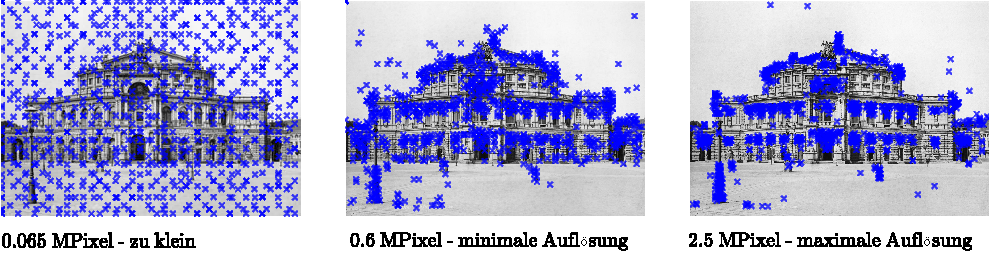
\includegraphics[scale=0.955]{scale_descriptor_selection.pdf}
\caption{Referenzpunkte der ausgewählten Deskriptoren bei unterschiedlicher Eingangsauflösung.}
\label{small_img}
\end{figure}
Auch sehr große Bilder können zu Problemen führen. Da die Bilder während dem Extraktionsprozess in mehreren Skalen betrachtet werden, können bei sehr großen Bildern Speicherproblem auftreten. Aus diesem Grund wird für die Bilder des Datensatzes eine minimale Auflösung von $0.6$MPixel und eine maximale Auflösung von $2.5$MPixel gefordert. Bilder die diese Restriktionen über- bzw. unterschreiten, werden auf die Maximal- bzw. Mindestgröße skaliert.\\
Neben historischen Daten wird das DELF-Verfahren zusätzlich auf dem Oxford5k-Datensatz \cite{oxford5k} getestet (vgl. Tab. \ref{oxford5k_data}). Hierbei handelt es sich um einen häufig verwendeten Benchmarkdatensatz, bestehend aus $5063$ Bildern. Das Bildmaterial entstammt Suchanfragen zu $11$ unterschiedlichen Sehenswürdigkeiten in und um Oxford, an die Fotocommunity Flickr\footnote{\url{https://www.flickr.com/}, zuletzt besucht am 03.09.20}. Häufig finden sich dabei Bilder von Personen oder Aufnahmen von Innenräumen, die keine der gesuchten Sehenswürdigkeiten abbilden. Diese Störbilder können entweder als zusätzliche Herausforderung angesehen oder aber vorab aussortiert werden. In den in dieser Arbeit durchgeführten Experimenten sind diese Störbilder im Datensatz enthalten. 
\begin{table}[h]
\centering
\begin{tabular}{l|c|c|c|c}
\rowcolor[HTML]{C0C0C0} 
Objekt                 & Radcliffe Camera & Christ Church & All Souls   & Magdalen \\
Anzahl Objektimpressionen & 348              & 133           & 111         & 103      \\
Anzahl Anfragen           & 5                & 5             & 5           & 5        \\ \hline
\rowcolor[HTML]{C0C0C0} 
Objekt                & Hertford         & Ashmolean     & Bodleian    & Balliol  \\
Anzahl Objektimpressionen & 61               & 31            & 30          & 18       \\
Anzahl Anfragen           & 5                & 5             & 5           & 5        \\ \hline
\rowcolor[HTML]{C0C0C0} 
Objekt                 & Cornmarket       & Keble         & Pitt Rivers & Total    \\
Anzahl Objektimpressionen & 13               & 11            & 8           & 867      \\
Anzahl Anfragen           & 5                & 5             & 5           & 55       \\ \hline
\rowcolor[HTML]{C0C0C0} 
Impressionen pro Bild     & 0                & 1             & 2           & Total    \\
Anzahl Bilder             & 4218             & 823           & 22          & 5063    
\end{tabular}%
\caption{Aufbau des Oxford5k Datensatzes}
\label{oxford5k_data}
\end{table}

\section{Retrievalmetriken}

Obwohl sich Klassifikations- und Retrievalaufgaben im Kern ähneln, können viele Metriken mit denen Klassifikationssysteme üblicherweise bewertet werden, wie beispielsweise Genauigkeit, nicht verwendet werden, um die Performanz von Retrievalsystemen zu evaluieren. Generell lassen sich aus der Betrachtung einzelner Bildpaare bestehend aus Anfragebild und Bildern des Suchindexes keine Rückschlüsse über die Performanz von Retrievalsystems ziehen.  Grundlage der Bewertung sind stets die gesamten Antworten des Retrievalsystems auf eingehende Suchanfragen. Entscheidend sind hierbei die Rankings, bzw. die Reihenfolgen in der die Bilder des Suchindexes auf die Anfragen zurückgegeben werden. Eine Möglichkeit diese Reihenfolgen zu bewerten ist die Erstellung sogenannter ROC-Kurve (Reciever-Operating-Characteristic)(vgl. Abb. \ref{metric_curve}a). Hierfür wird jeweils eine wachsender Anteil der zurückgegeben Bilder betrachtet und das Verhältnis zwischen Richtig-Positiv-Rate bzw. Recall und Falsch-Positiv-Rate dargestellt. Der Recall gibt an, welcher Anteil an Bildern mit gewünschten Bildinhalt bereits im betrachteten Abschnitt der Rückgabe enthalten war.
\begin{equation}
\text{Recall} = \frac{|\text{Bereits züruckgebene Bilder mit gewünschtem Inhalt}|}{|\text{Im Datensatz enthaltene Bilder mit gewünschtem Inhalt}|}
\end{equation}
Analog beschreibt die Falsch-Positiv-Rate den Anteil der Bilder ohne gewünschten Bildinhalt, der bereits zurückgegeben wurde.
\begin{equation}
\text{Falsch-Positiv-Rate} = \frac{|\text{Bereits züruckgebene Bilder ohne gewünschtem Inhalt}|}{|\text{Im Datensatz enthaltene Bilder ohne gewünschtem Inhalt}|}
\end{equation}
\begin{figure}[h]
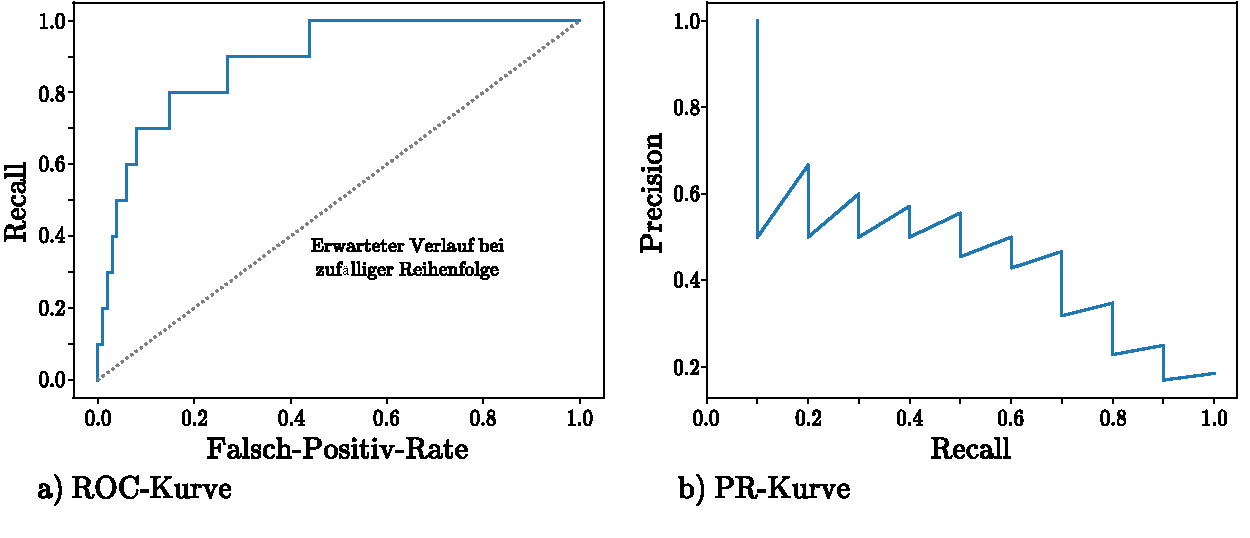
\includegraphics[scale=0.76]{metric_curves.pdf}
\caption{Vergleich von Kurvenmetriken einem Beispielsranking}
\label{metric_curve}
\end{figure}
\\
ROC-Kurven beginnen stets im Ursprung, wo noch keine Bilder zurückgegeben wurden und enden im Punkt $(1,1)$ wo der gesamte Datensatz zurückgegeben wurde. Die Gerade zwischen diesen Punkten bildet den erwarteten Verlauf, wenn das System Bilder in einer zufälligen Reihenfolge zurückgibt. Ein Retrievalsystem hat nur dann einen positiven Effekt für den Nutzer, wenn die ROC-Kurven ihrer Anfrageantworten oberhalb dieser Linie verlaufen. Obwohl ROC-Kurven gut in der Lage sind den Unterschied eines Suchsystems gegenüber einer zufälligen Suche aufzuzeigen, vermitteln sie aus der Perspektive eines tatsächlichen Anwenders oft ein zu positives Bild der Ergebnisse. Das liegt daran, dass der Anteil der Bilder, die für eine Anfrage relevant sind meist um ein vielfaches kleiner ist als der Anteil der irrelevanten Bilder, was an einer ROC-Kurve jedoch nicht ablesbar ist. Angenommen für eine Suchanfrage sind $10\%$ eines durchsuchten Datensatzes tatsächlich relevant und die zur Anfrageantwort erstellte ROC-Kurve zeigt bei einem Recall von $90\%$ eine Falsch-Positiv-Rate von $30\%$. Obwohl der Verlauf der Kurve ein sehr gutes Ergebnis suggeriert, sind für den Nutzer $75\%$ der zurückgegebenen Bilder irrelevant, die er gesehen hat, bevor ein Recall von $90\%$ erreicht wurde. Eine Möglichkeit, die tatsächliche Nutzererfahrung besser abzubilden ist die Erstellung von sogenannten PR-Kurven (Precision-Recall) (vgl. Abb. \ref{metric_curve}b). Hierbei wird die Präzision, also der Anteil der relevanten Bildern in der bisherigen Rückgabe gegen den Recall abgebildet.
\begin{equation}
\text{Precision} = \frac{|\text{Bereits züruckgebene Bilder mit gewünschtem Inhalt}|}{|\text{Bereits züruckgebene Bilder}|}
\end{equation}
So kann direkt abgelesen werden, welchen Anteil an irrelevanten Bildern innerhalb der Rückgabe toleriert werden müssen, um einen bestimmten Anteil der gesuchten Bilder zu finden.
Die vorgestellten Kurvenmetriken eigenen sich gut um einzelne Anfragen an Retrievalsysteme zu analysieren und zu visualisieren. Um Retrievalsysteme in Gänze, auf Basis mehrerer Anfrage zu bewerten und mit anderen Systemen zu vergleichen, bietet es sich an ein kompaktere Metriken zu verwenden. Hierfür wird können die Flächen unterhalb der Metrikkurven betrachtet werden. AUC (Area Under Curve) und AP (Average Percision) beschrieben jeweils die Flächen unterhalb von ROC bzw. PR-Kurven und können so eine Anfrageantwort mit einer einzelnen Zahl bewerten. Auf Grund der besseren Beschreibung des Nutzererlebnisses werden in dieser Arbeit PR-Kurven bzw. AP-Werte zur Auswertung genutzt. Für den Vergleich zwischen unterschiedlichen Retrievalsystemen oder Konfigurationen von DELF werden die AP-Werte von mehreren Anfragen an ein System zu einem Mittelwert (mAP) zusammengefasst. So kann die Performanz eines Retrievalsystems in einer einzelnen Zahl dargestellt werden. 
 

\section{Parameter Analyse}

Ein wesentliches Ziel dieser Arbeit ist es das DELF-Verfahren insbesondere für den Anwendungsfall des Retrievals von historischen Abbildungen zu optimieren. Hierfür werden ein Reihen an Parametern entlang der DELF-Pipeline variiert und ihre Einflüsse, auf die Retrievalergebnisse analysiert. Um belastbare Aussagen über die Einflüsse einzelner Parameter machen zu können, muss eine große Anzahl unterschiedlicher Parameterkonfigurationen betrachtet und Experimente diesbezüglich mehrfach wiederholt werden. Die dafür benötigte Rechenleistung ist sehr groß und auf einem normalen Desktopsystem nicht innerhalb des Zeitrahmens einer Masterarbeit realisierbar.\\
Die Experimente werden daher auf dem HPC-DA System\footnote{\url{https://tu-dresden.de/zih/hochleistungsrechnen/hpc}} des Zentrums für Informationsdienste und Hochleistungsrechnen (ZIH), der TU Dresden durchgeführt. Die verwendete Partition für maschinelles Lernen besteht aus $32$ Knoten, mit jeweils $6$ NVIDIA VOLTA V100 GPUs und $2$ IBM Power9 CPUs mit je $22$ Kernen. Die große Anzahl an leistungsstarken Rechenknoten erlaubt es viele unterschiedliche Konfigurationen parallel und zügig zu untersuchen.
In Tab.\ref{hpc} findet sich eine Übersicht der rechenintensiven Experimentreihen, die im Zuge dieser Arbeit durchgeführt wurden, mit Informationen über verwendete Hardware und benötigter Rechenzeit.

\begin{table}[h]
\resizebox{\textwidth}{!}{%
\begin{tabular}{|l|l|l|l|l|l|l|}
\hline
\rowcolor[HTML]{C0C0C0} 
Experiment                                                                             & \#Läufe & \#CPU-Kerne & \#GPUs & Totale Laufzeit (h) & Totale CPU-Zeit (h) & Totale GPU-Zeit (h) \\ \hline
\begin{tabular}[c]{@{}l@{}}Hyperparameteroptimiertung\\ Finetuning\end{tabular}        & $1$     & $10$        & $10$   & $16$                & $160$               & $160$               \\ \hline
\begin{tabular}[c]{@{}l@{}}Hyperparameteroptimierung\\ Attention-Training\end{tabular} & $2$     & $48$        & $12$   & $40$                & $1920$              & $480$               \\ \hline
Modelltraining                                                                         & $12$    & $2-3$       & $1$    & $78$                & $226$               & $78$                \\ \hline
Retrievalexperimente                                                                   & $919$   & $30$        & $1$    & $2027$              & $60834$             & $2027$              \\ \hline
\multicolumn{4}{|l|}{Summe}                                                                                             & $2325$              & $63140$             & $2745$              \\ \hline
\end{tabular}%
}
\caption{Übersicht über rechenintensive Experimente, durchgeführt auf der ML-Partition des HPC-DA Systems. Rechenzeiten sind jeweils über alle Läufe einer Experimentalreihe summiert. CPU-Zeit bezieht sich auf die akkumulierte Rechenzeit der CPU-Kerne.}
\label{hpc}
\end{table}

\subsection{Hyperparameteroptimierung der Trainingsphasen}\label{hyperparam}
Die ersten Experimentalreihen befassen sich mit den Trainingsphasen des DELF-Verfahrens. Um bei späteren Retrievalversuchen gute Ergebnisse erzielen zu können, benötigt man Modelle die in der Lage sind aussagekräftige Bildrepräsentationen zu erstellen. Für die Experimente zum Modelltraining wird dabei angenommen, dass die Güte, der von einem Modell erzeugten Deskriptoren bzw. der von einem Modell getroffenen Auswahl an Deskriptoren positiv mit der Fähigkeit, der Modelle korreliert die beim Training gestellte Klassifikationsaufgaben zu lösen. Um die Modelle zu bewerten wird daher der Fehler, in Form der Kreuzentropie betrachtet, der auftritt wenn das Modell einen Validierungsdatensatz klassifiziert. Vor Beginn jedes Experiments werden zufällig $20\%$ der Trainingsbilder (siehe Kap. \ref{trainingsdata} auf Seite \pageref{trainingsdata}) für die Validierung ausgewählt. Die Validierungsdaten stehen dem Modell während des Trainingsprozesses nicht zur Verfügung. Daher können sie genutzt werden, um zu überprüfen, ob ein Modell auch auf ungesehenen Daten vergleichbare Ergebnisse erzielt.
\\
Der Erfolg des Trainingsprozesses hängt wesentlich von der zu trainierenden Architektur und der vorhandenen Datenlage ab. Einfluss haben außerdem Parameter, die den Ablauf des Trainingsprozesses beeinflussen. Die Experiments, die in diesem Abschnitt besprochen werden befassen sich mit der Suche nach optimalen Werten für drei dieser sogenannten Hyperparameter. Betrachtet wird die Anzahl der Trainingsepochen, die Lernrate, die bestimmt wie stark Netzwerkparameter in einem Optimierungsschritt angepasst werden, sowie der Faktor $\gamma$ mit dem die Lernrate alle $10$ Epochen multipliziert wird\footnote{Als weiterer Hyperparameter wird weight decay untersucht, allerdings lässt sich hier kein signifikanter Einfluss auf den Validierungsfehler feststellen. Die Ergebnisse hierzu finden sich im Anhang ab Seite \pageref{weight_decay}}. Die übrigen Hyperparameter sind für alle Experimente fest gesetzt. Die Modelle werden mit einer Batchgröße von $8$ trainiert und mittels Stochastic Gradient Decent (kurz SGD \footnote{\url{https://pytorch.org/docs/stable/optim.html\#torch.optim.SGD}, zuletzt besucht am 30.07.20}) optimiert. Für die zu untersuchenden Hyperparameter werden jeweils Wertebereiche definiert. Die Länge des Trainings kann zwischen $10$ und $40$ Epochen dauern. Die initiale Lernrate wird zwischen $0.01$ und $0.001$ gewählt und der $\gamma$-Faktor liegt im Bereich zwischen $1$ und $0.1$.
\\
Um den Suchraum effizient erkunden zu können wird das von Norman Koch entwickelte NNOPT-Tool verwendet, um neue Hyperparameterkonfigurationen zu erstellen und auf dem HPC-System zu testen. Das NNOPT-Tool, das auf dem Hyperopt-Paket \cite{hyperopt} von Bergstra, Yamins und Cox basiert, wählt automatisch Werte für die zu untersuchenden Hyperparameter innerhalb der definierten Wertebereiche aus und startet mit diesen Experimente auf dem Großrechner. Ist ein Experiment abgeschlossen erhält NNOPT zur Bewertung der Konfiguration den erzielten Validierungsfehler. Neue Konfigurationen werden bevorzugt in der Nähe von bereits getesteten Konfigurationen erstellt, die gute Ergebnisse erzielt haben. Dies erlaubt es schneller optimale Hyperparameterwerte zu finden, als mit einer zufälliger Suche.
\\
Für das Fine-Tuning wurden auf diese Art $22$ unterschiedliche Konfigurationen getestet. Es lässt sich beobachten, dass fast alle getesteten Konfigurationen Modell erzeugen, die in der Lage sind die Trainingsaufgabe sehr gut zu lösen. Im Schnitt erzielen die trainierten Modelle eine Klassifikationgenauigkeit von $95.13\%$ auf den Validierungsdaten\footnote{Obwohl zum Vergleich der Konfigurationen der Validierungsfehler berechnet wurde, wird die Modellperformanz im Folgenden über die Validierungsgenauigkeit dargestellt, da diese Metrik intuitiver ist.}, wobei $20$ der $22$ Modelle eine Genauigkeit von über $90\%$ erreichen(vgl. Abb.\ref{finetuning_int_end}b). Da auf Grund der guten Ergebnisse nur wenig Potential für Verbesserung besteht und die beobachtet Varianz der Ergebnisse unterschiedlicher Konfigurationen gering ist, werden keine weiteren Testläufe zur Hyperparameteroptimierung durchgeführt. Es sei jedoch erwähnt, dass sich auf Grund der im Verhältnis zu Größe der Suchraumes geringen Anzahl an Testläufen keine eindeutigen Abhängigkeiten zwischen Hyperparametern und Klassifikationsperformanz ableiten lassen.
\\
Gut beobachten lässt sich der positive Effekt der Nutzung eines vortrainierten Modells zu Initialisierung der Netzwerkparameter. So erreichen alle getesteten Konfigurationen bereits nach der ersten Trainingsepoche eine Validierungsgenauigkeit von über $85\%$ (vgl. Abb.\ref{finetuning_int_end}a). Die initialisierten Parameter müssen nur noch geringfügig angepasst werden, um die neue Trainingsaufgabe zu lösen, weshalb die Modelle von Beginn an gute Ergebnisse erzielen. 
\\
\begin{figure}[h]
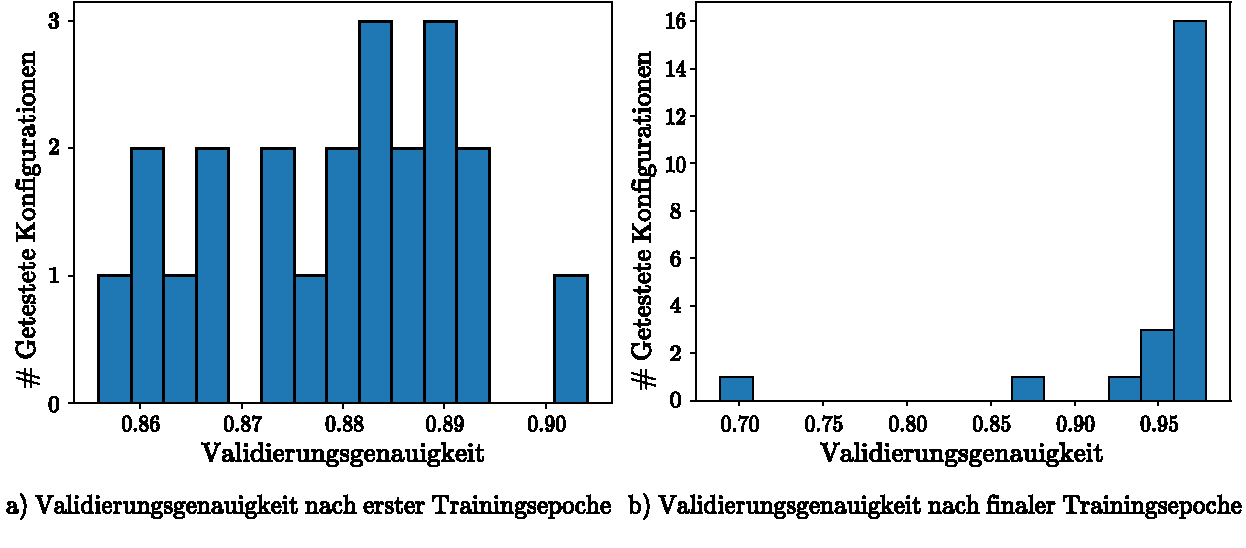
\includegraphics[scale=0.750]{NNOPT/init_and_end_perf_finetuning.pdf}
\caption{Erreichte Klassifikationsgenaugikeit nach der ersten bzw. letzten Epoche des Fine-Tunings, der getesteten Konfigurationen. Achsenskalierung variiert.}
\label{finetuning_int_end}
\end{figure}
\\
Betrachtet man die Ergebnisse der Testläufe in Kombination mit den dazugehörigen Hyperparametern (siehe Abb.\ref{finetuning_all}), so scheint die Anzahl an Trainingsepochen keinen signifikanten Einfluss auf die erzielte Validierungsgenauigkeit zu haben. Dies deckt sich mit der Annahme, dass sich Netzwerkparameter mittles Fine-Tuning in wenigen Epochen optimieren lassen. Betrachtet man den Trainingsverlauf des Fine-Tunings (vgl. Abb. \ref{finetuning_lr_gamma_verlauf}), so stellt man fest, das für die meisten Konfigurationen nach $10-15$ Epochen keine großen Verbesserungen mehr im Hinblick auf die Validierungsgenauigkeit erzielt werden.  
\begin{figure}[h]
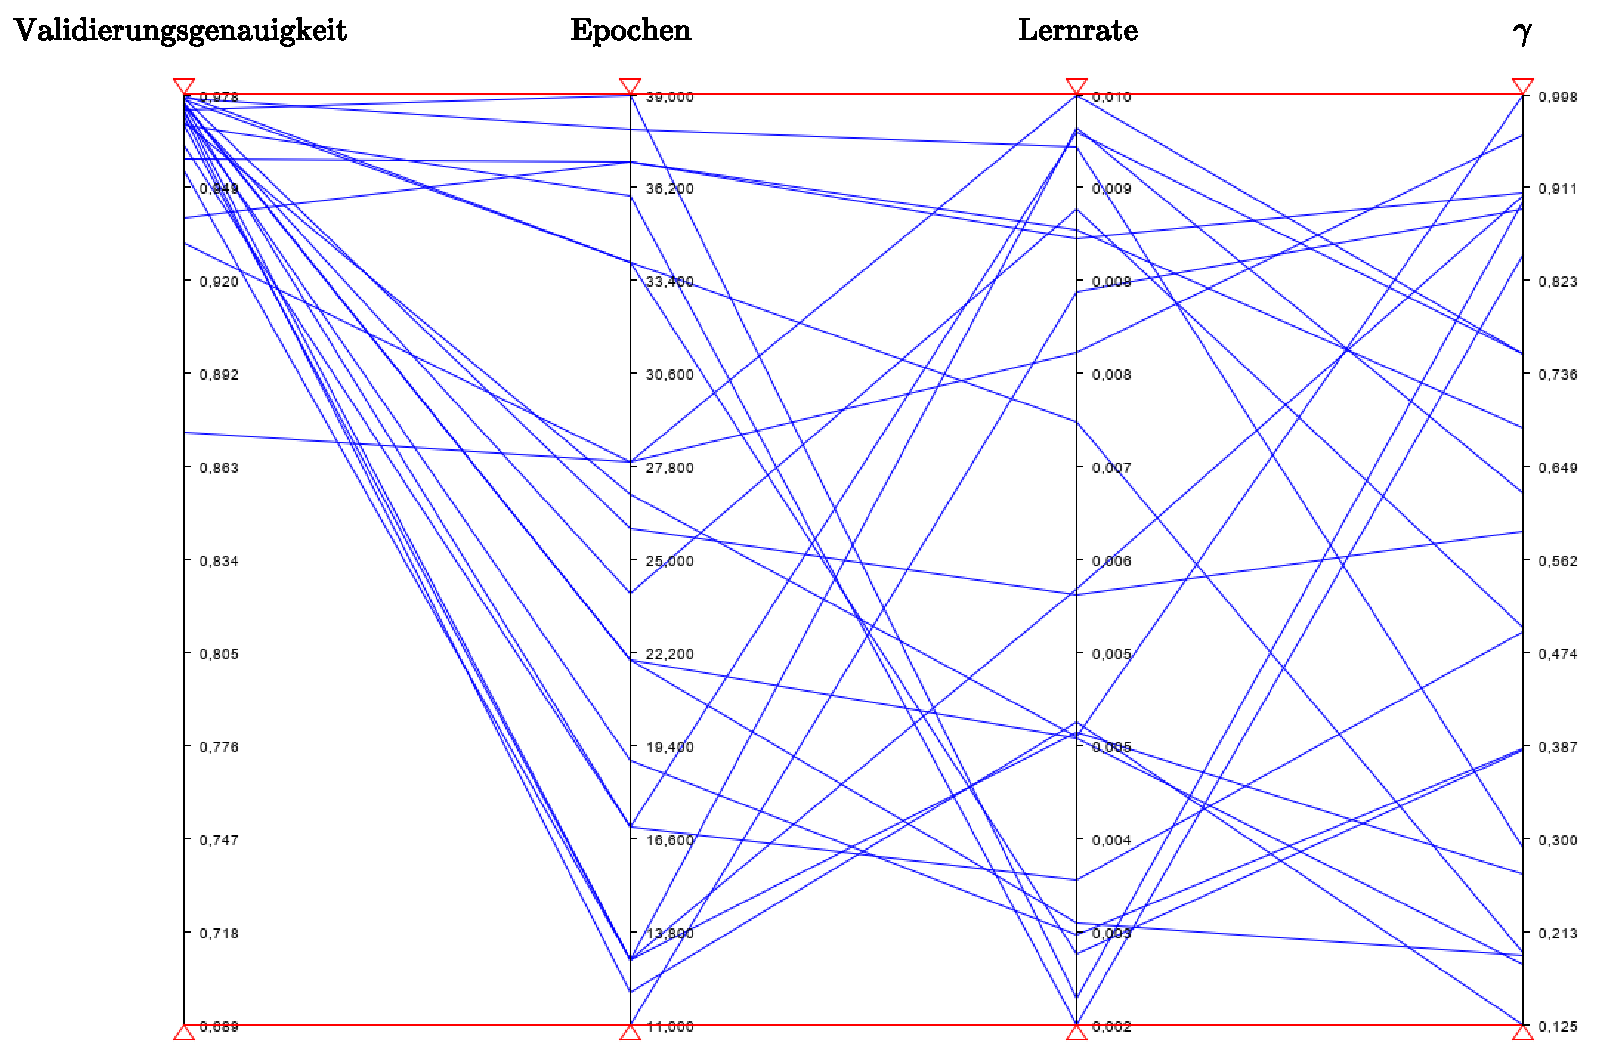
\includegraphics[scale=0.58]{NNOPT/finetuning_all.pdf}
\caption{Parallele Darstellung der getesteten Konfigurationen des Fine-Tunings. Jede Linie repräsentiert einen Konfiguration und die von ihr erzielte Validierungsgenauigkeit.}
\label{finetuning_all}
\end{figure}
\\
Beleuchtet man die in den getesteten Konfigurationen genutzten Lernraten, so stellt sich heraus, dass alle Testläufe mit einer Lernrate unter $0.005$ eine sehr gute Validierungsgenauigkeit erreichen. Werden höhere Lernraten genutzt, so unterscheiden sich die erzielten Ergebnisse deutlich stärker. Bezieht man die dazugehörigen $\gamma$-Faktoren mit ein, sieht man, dass Konfigurationen mit hoher Lernrate, aber niedrigem $\gamma$-Faktor, also mit starker Reduktion der Lernrate während des Trainingsverlaufes, ebenfalls sehr gute Ergebnisse erzielen. Läufe mit hoher Lernrate, sowie hohem $\gamma$-Faktor schneiden dagegen eher schlechter ab (Siehe Abb. \ref{finetuning_lr_gamma}). Analysiert man die Trainingsverläufe der unterschiedlichen Konfigurationen (Siehe Abb.\ref{finetuning_lr_gamma_verlauf}), findet sich eine mögliche Erklärung für diese Verhalten. Bei niedriger Lernrate nähert sich die Validierungsgenauigkeit ohne starke Einbrüche einem Maximum an. Ist die Lernrate hoch fluktuiert die Validierungsgenauigkeit jedoch stark. Dies weist darauf hin, dass die Modelle nicht in der Lage sind ein stabiles Optimum für ihre Parameter zu finden. Hohe Lernraten können dazu führen, dass Parameter bei Optimierungsschritten zu stark verändert werden und so ihr Optimum immer wieder überspringen. Nach Abschluss der ersten $10$ Epochen wird die Lernrate mit dem $\gamma$-Faktor multipliziert. Für Läufe mit hoher initialer Lernrate und niedrigem $\gamma$-Faktor lässt ab diesem Punkt ein gleichmäßigerer Lernprozess beobachten. 
\begin{figure}[h]
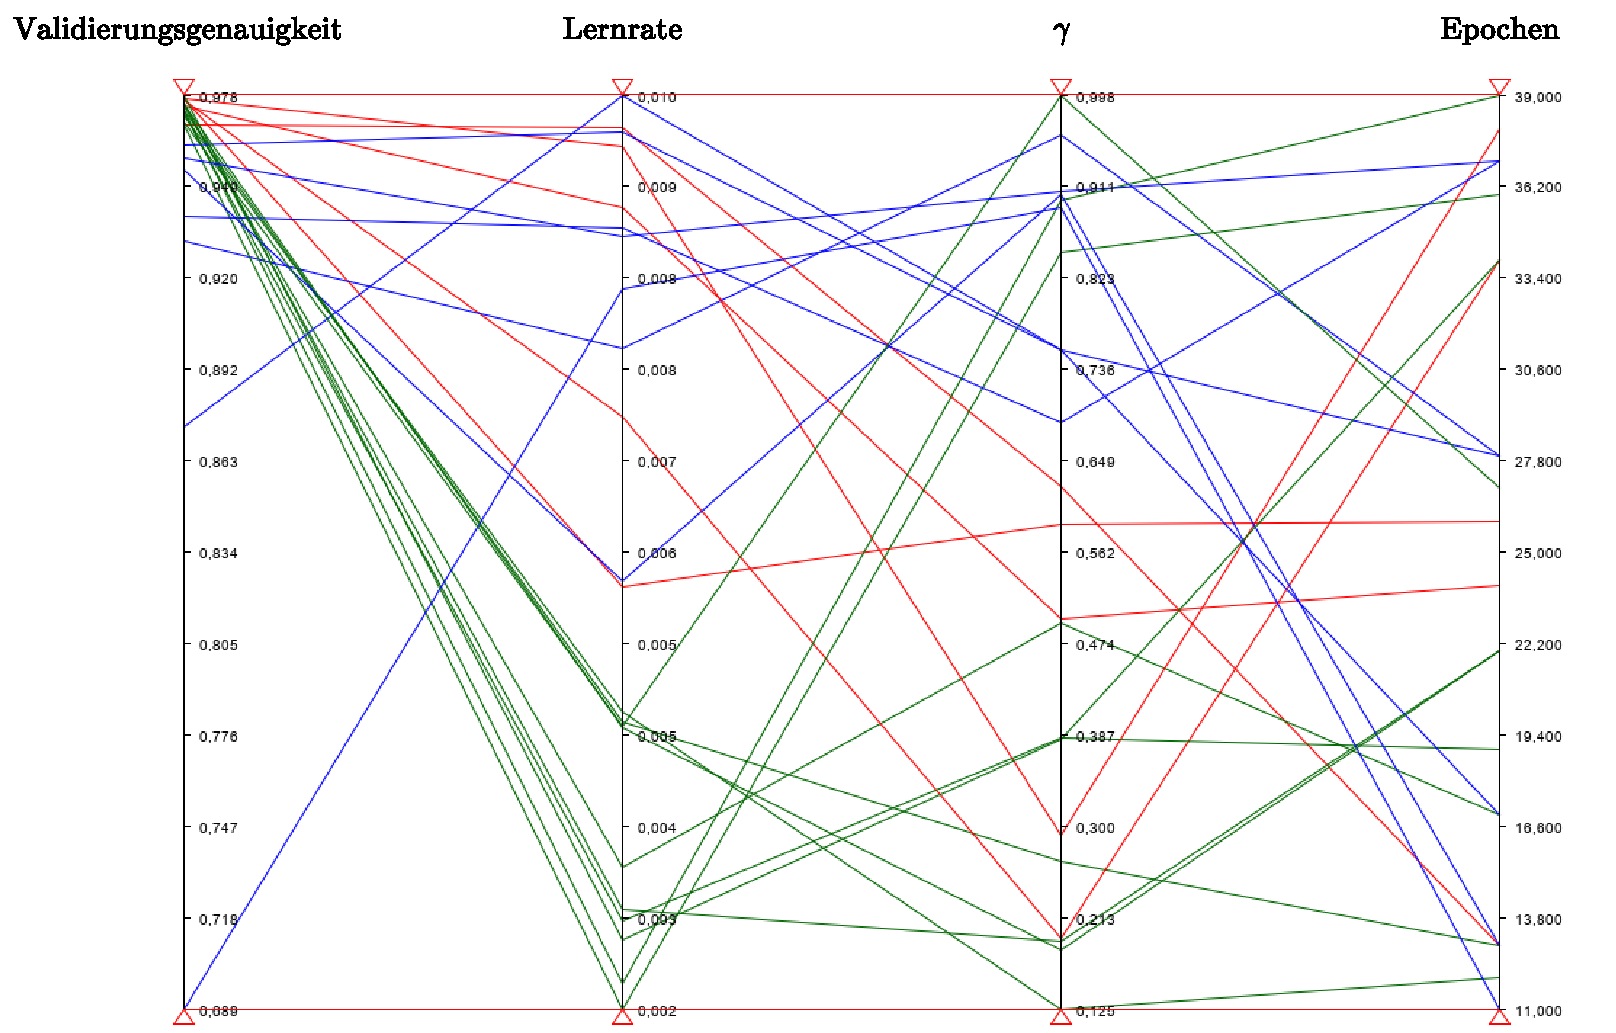
\includegraphics[scale=0.58]{NNOPT/finetuning_lr_gamma.pdf}
\caption{Betrachtung der genutzten Lernraten und $\gamma$-Faktoren. Grün: Konfigurationen mit niedriger Lernrate $(<0.005)$, Rot: Hohe Lernrate und niedriges $\gamma$ $(<0.65)$, Blau: Hohe Lernrate und hohes $\gamma$}
\label{finetuning_lr_gamma}

\centering
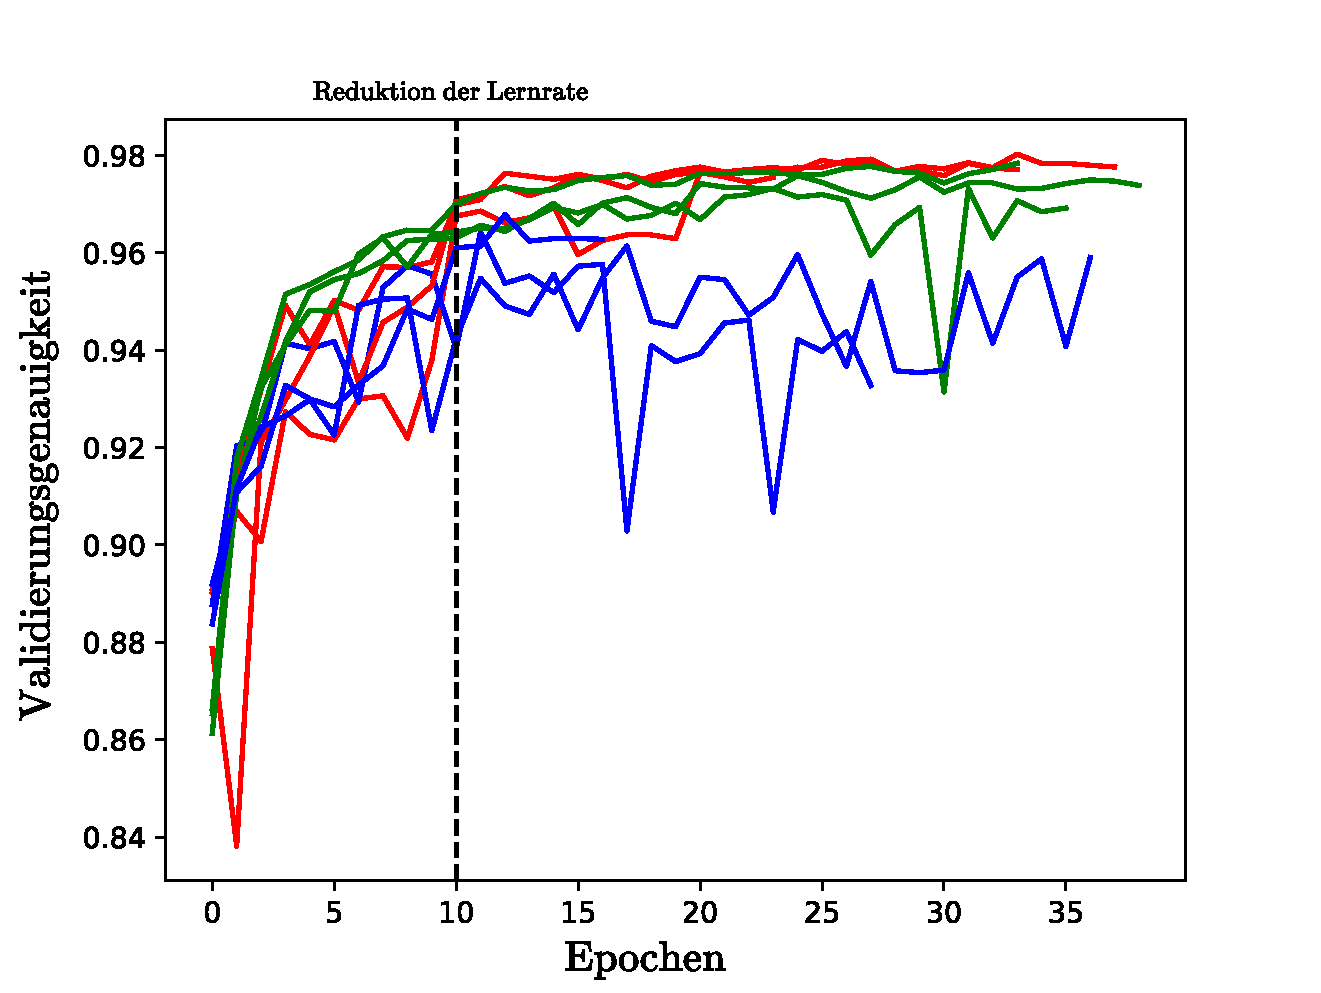
\includegraphics[scale=1]{NNOPT/finetuning_lr_gamma_verlauf.pdf}
\caption{Trainingsverlauf der Fine-Tunings, bei unterschiedlicher Lernrate und $\gamma$. Farbgebung analog zu Abb.\ref{finetuning_lr_gamma}}
\label{finetuning_lr_gamma_verlauf}
\end{figure}
\clearpage
Die Konfiguration mit dem besten Trainingsergebnis schreibt eine Trainingsdauer von $22$ Epoche, bei einer initialen Lernrate von $0.0032$ und einem $\gamma$-Faktor von $0.19$ vor und erzielt nach der letzten Epoche eine Validierungsgenauigkeit von $97.6\%$.
\\
Das dabei trainierte Modell ist der Ausgangspunkt für die Hyperparameteroptimierung des Attention-Trainings. Analog wie in den Experimenten zum Fine-Tuning werden mit Hilfe von NNOPT $60$ unterschiedliche Konfigurationen für das Attention-Training getestet. Obwohl das Modell für das Attention-Training durch Entfernung des vierten ResNet-Blocks deutlich verkleinert wird und die Ausgaben des ResNets unter Verwendung des gewichteten Sum-Poolings (vgl. Abb.\ref{attention} auf Seite \pageref{attention}) sehr restriktiv genutzt werden, sind die Attention-Modelle in fast allen untersuchten Konfigurationen in der Lage die Klassifikationsaufgaben weiterhin sehr gut zu Lösen. So werden in $59$ der $60$ untersuchten Konfigurationen eine abschließende Validierungsgenauigkeit von über $89\%$ erreicht (siehe Abb.\ref{attention_int_end}b). Die durchschnittliche Validierungsgenauigkeit nach der letzten Trainingsepoche beträgt $91.3\%$, was einer durchschnittlichen Verschlechterung von $6.3\%$ gegenüber dem verwendeten fine-getunten ResNet-Modell entspricht. Im Kontrast zum Fine-Tuning variiert die gemessene Validierungsgenauigkeit nach der ersten Trainingsepoche der Attention-Trainings deutlich stärker und ist allgemein niedriger (vgl. Abb.\ref{attention_int_end}a). Da die Parameter der zu optimierenden Attention-Einheit nicht vortrainiert sind und daher zufällig initialisiert werden sind größere Unterschiede und schlechter Ergebnisse zu Beginn des Trainings, sowie eine längere benötigte Trainingsdauer zu erwarten.
\begin{figure}[h]
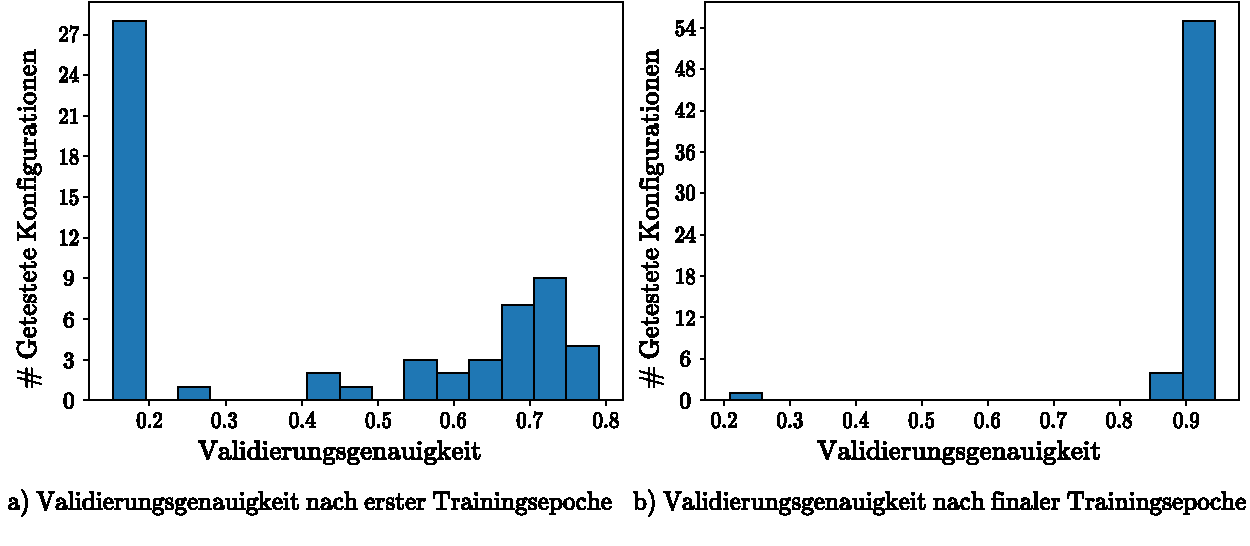
\includegraphics[scale=0.75]{NNOPT/init_and_end_perf_attention.pdf}
\caption{Erreichte Klassifikationsgenaugikeit nach der ersten bzw. letzten Epoche des Attention-Trainings, der getesteten Konfigurationen. Achsenskalierung variiert.}
\label{attention_int_end}
\end{figure}
\\
Betrachtet man die genutzte Anzahl an Trainingsepochen in Kombination mit der erreichten Validierungsgenauigkeit(siehe Abb.\ref{attention_epochs}), bestätigt sich diese Annahme. Konfigurationen mit einer Trainingsdauer unter $20$ Epochen erzielen in unseren Experimente durchschnittlich eine geringere Validierungsgenauigkeit. Ab mehr als $20$ Epochen schwächt sich der positive Effekt einer längeren Trainingsdauer jedoch deutlich ab.
\\
\begin{figure}[h]
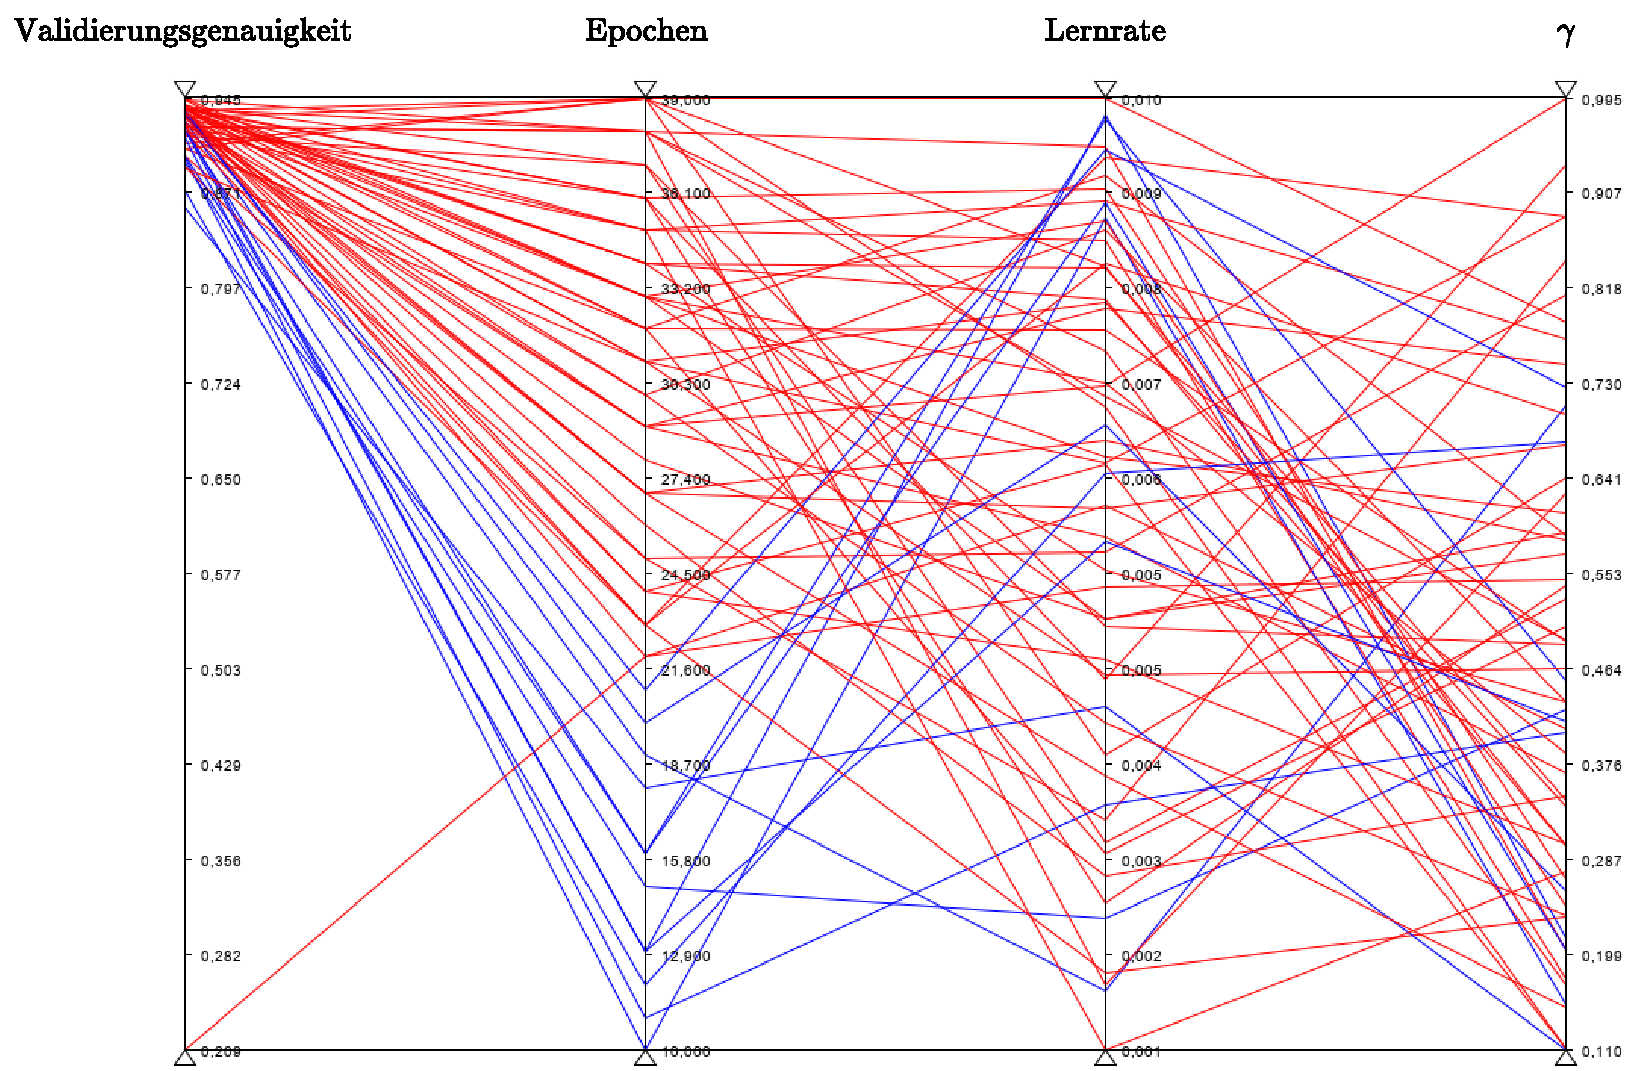
\includegraphics[scale=0.58]{NNOPT/attention_epochs.pdf}
\caption{Betrachtung der gewählten Trainingsdauer. Rot: Über $20$ Epochen, Blau: $20$ oder weniger Epochen}
\label{attention_epochs}
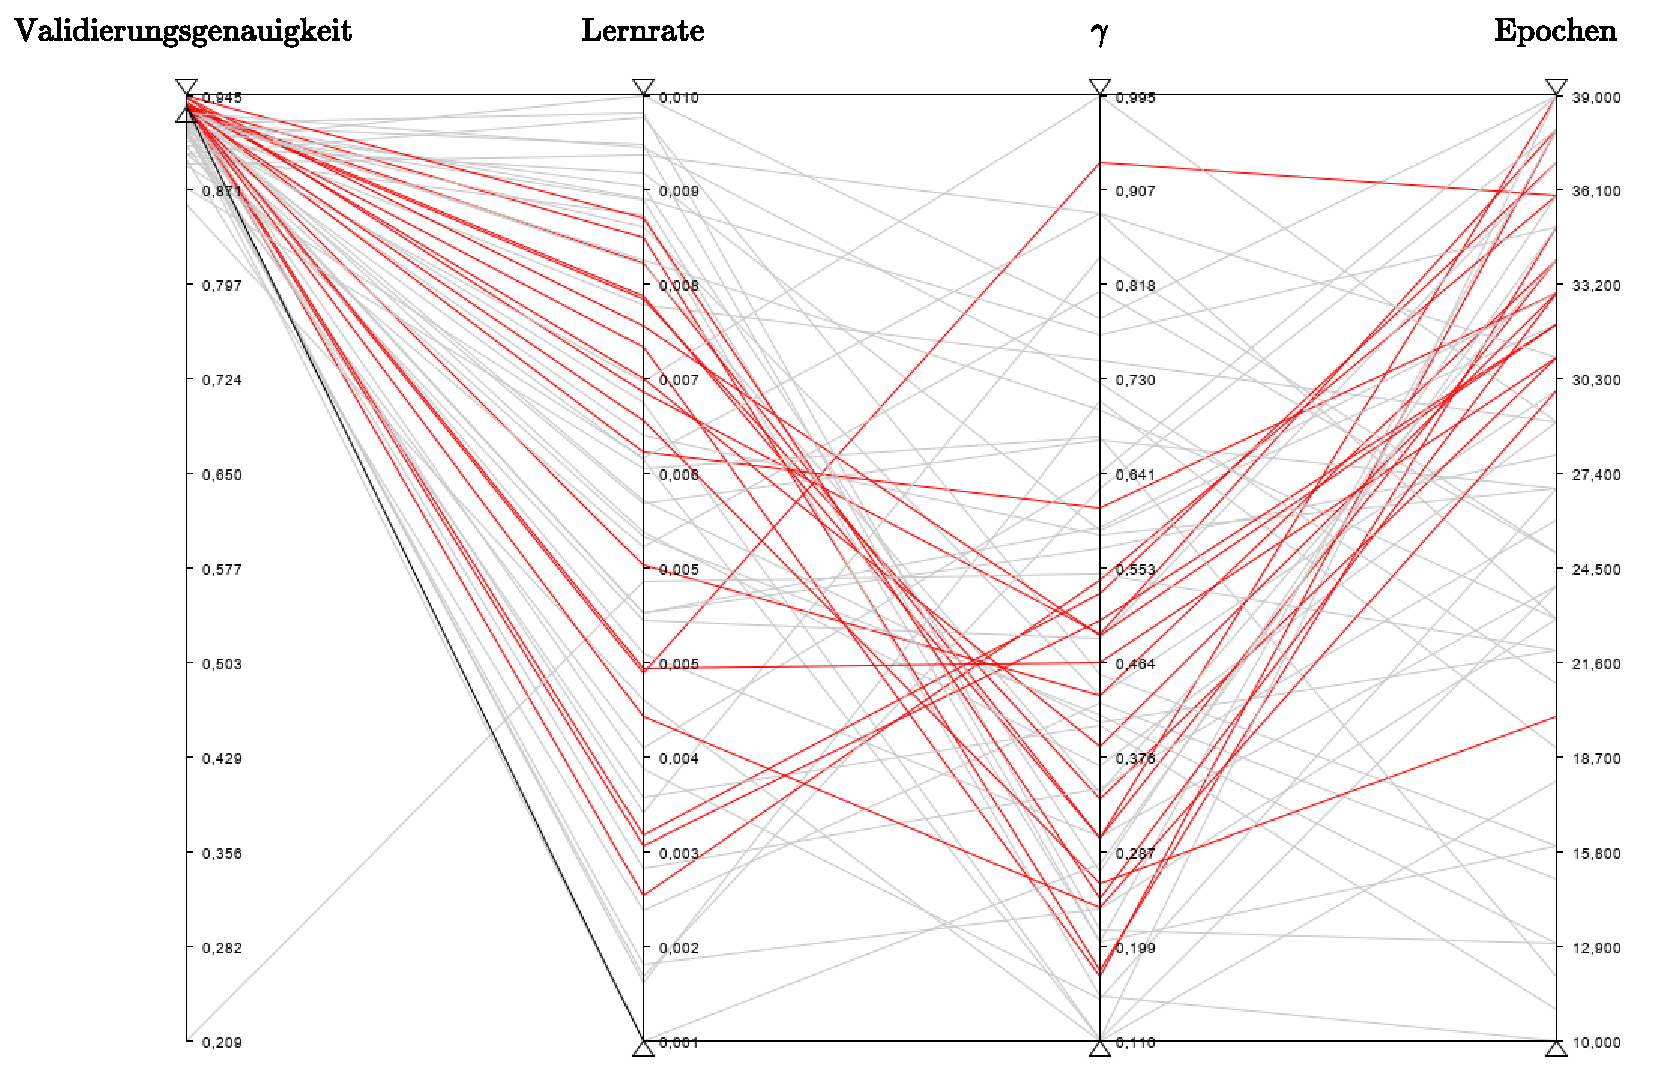
\includegraphics[scale=0.58]{NNOPT/attention_top_runs.pdf}
\caption{Darstellung der Validierungsgenauigkeit nach Trainingsende. Rot: Läufe mit Validierungsgenauigkeit $\geq 93.5\%$, Grau: Läufe mit niedrigerer Validerungsgenauigkeit}
\label{attention_top}
\end{figure}
\clearpage
Für Lernrate und $\gamma$-Faktor lassen sich nur schwer Tendenzen erkennen. Über den gesamten Suchraum dieser Parameter lassen sich sowohl Konfigurationen mit hoher, sowie Konfigurationen mit weniger hoher Validierungsgenauigkeiten erreichen finden. Die Konfigurationen, welche die höchsten Validierungsgenauigkeiten erreichen (Siehe Abb.\ref{attention_top}) nutzen jedoch alle eine Lernrate im Bereich zwischen $0.0025$ und $0.009$. Die $\gamma$-Faktoren dieser Konfigurationen liegen meist unter $0.55$ und die Trainingsdauer über $30$ Epochen.
Die beste gefundene Konfiguration erzielt eine Validierungsgenauigkeit von $94.5\%$ und nutzt dabei eine Lernrate von $0.0078$ einen $\gamma$-Faktor von $0.49$ und eine Trainingslänge von $32$ Epochen. 
Mit Hilfe der ermittelten Hyperparameterwerte der besten gefundenen Konfigurationen für Fine-Tuning und Attention-Training werden $6$ neue Modelle Trainiert, die in den Retrievalexperimenten zur Extraktion der Deskriptoren genutzt werden. Die Trainingsverläufe dieser Modelle sind in Abb.\ref{optimized_runs} dargestellt.
\begin{figure}[h]
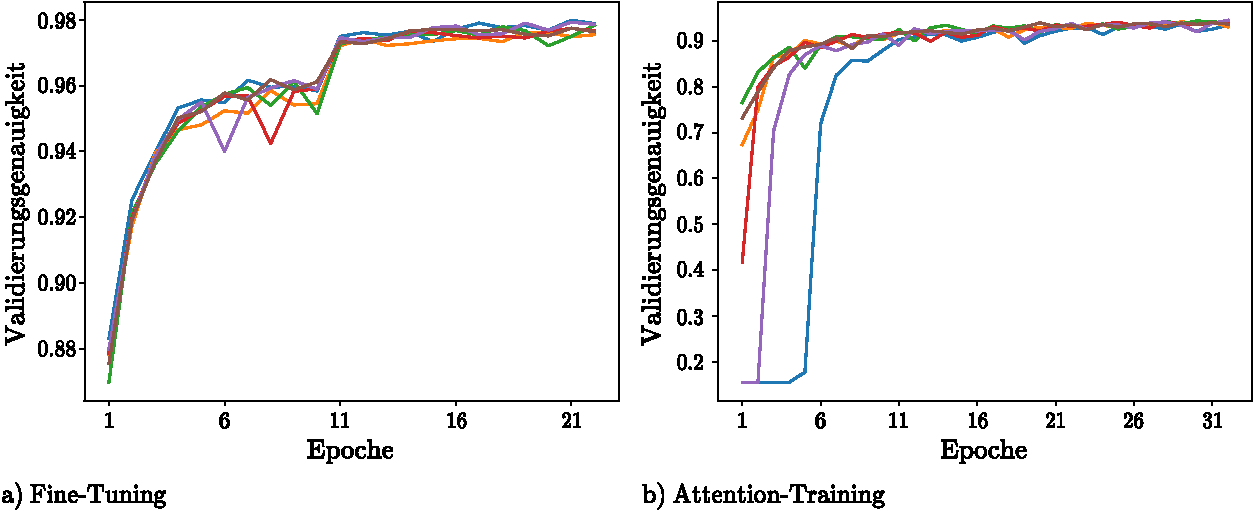
\includegraphics[scale=0.75]{NNOPT/6_model_verlauf}
\caption{Trainingsverläufe mit optimierten Hyperparametern. Gleichefarbige Linen gehören zu gemeinsamen Trainingsläufen. Achsenskalierung variiert.}
\label{optimized_runs}
\end{figure}

\subsection{Variieren der Deskriptorlänge}\label{pca_experiments}

Nach Betrachtung der Trainingsphasen und Erstellung optimierter Modelle, werden nun Parameter aus den späteren Phasen des Verfahrens untersucht.
Ein zentraler Parameter der Extraktions- und Verarbeitungsphase ist die Anzahl an Dimensionen, der Deskriptoren nach der Transformation mittels Hauptkomponentenanalyse (vgl. \ref{pca_chapter} auf Seite \pageref{pca_chapter}). Da die zu einem Suchdatensatz erstellte Repräsentation fast ausschließlich aus den transformierten Deskriptoren besteht, sind diese für den überwiegenden Teil des Speicherbedarfs verantwortlich, der während der aktiven Verwendung des Suchsystems anfällt \footnote{Bei der Suche nach den ähnlichsten Deskriptoren während dem Matching hat die Deskriptorlänge auch einen Einfluss auf die Laufzeit. Da der Rechenaufwand für die geometrische Verifizierung von Matches, die nicht von der Deskriptorlänge abhängt, jedoch deutlich größer ist, ist dieser Einfluss vernachlässigbar.}. Insbesondere bei der Suche in großen Datenbanken ist es daher notwendig die Deskriptoren stark zu komprimieren. Durch die verwendete Art der Komprimierung geht jedoch auch immer ein Teil der ursprünglich in den Deskriptoren enthaltenen Informationen verloren. Es wird erwartet, dass sich der Informationsverlust durch die Deskriptortransformation negativ auf die Qualität des initialen Deskriptormatchings auswirkt. Um diesen Informationsverlust zu quantifizieren wird der Anteil der ursprünglichen Varianz zwischen den Deskriptoren errechnet, die nach der Transformation erhalten bleibt. Hierbei werden alle Deskriptoren betrachtet, die für die Berechnung der Hauptkomponentenanalyse genutzt wurden. Es ist davon auszugehen, dass sich der Informationsverlust auf unbeteiligten Deskriptoren ähnlich verhält. Die Autoren des DELF-Papiers \cite{delf} schlagen als Kompromiss zwischen erhaltener Information und Kompaktheit vor die Deskriptoren auf $40$ Dimensionen zu reduzieren. Wie dieser Wert ermittelt wurde wird jedoch nicht beschrieben. Um eine geeigneten Anzahl an Dimensionen zu ermitteln werden neben der von den Autoren empfohlenen Anzahl auch die Hälfte bzw. ein Vielfaches an erhaltenen Dimensionen, bis zu $200$ getestet. In Abb. \ref{explained_variance_ratio} wird der Einfluss der Deskriptorlänge auf den Anteil der erklärten ursprünglichen Varianz dargestellt.
\begin{figure}[h]
\centering
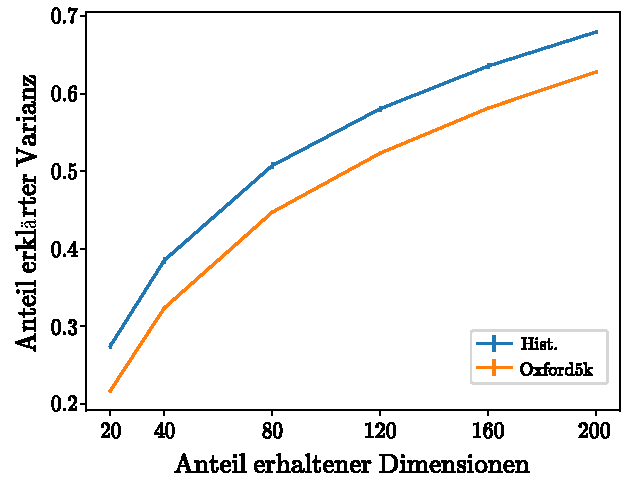
\includegraphics[scale=1]{explained_variance.pdf}
\caption{Erklärter Anteil der Varianz nach Deskriptortransformtion durch Hauptkomponentenanalyse auf unterschiedlichen Retrievaldatensätzen, je nach Anzahl erhaltener Dimensionen.}
\label{explained_variance_ratio}
\end{figure}
Die Variation der Deskriptorlänge hat nicht nur Einfluss darauf, welche Deskriptorpaare während dem initialen Matching bestimmt werden, sondern auch wie groß die euklidische Distanz zwischen diesen Paaren ist. Die Deskriptoren werden vor dem Matching zwar Längennormiert, sodass der maximale Abstand zwischen Deskriptoren $2$ beträgt. Der mittlere Abstand der bestimmten Deskriptorenpaare ist jedoch von der Varianz zwischen den Deskriptoren abhängig und steigt daher mit wachsender Deskriptorlänge. Während dem initialen Deskriptormatching werden Matchingpaare, deren Abstand über einem Distanzschwellwert liegen verworfen, um inkorrekte Matches auszusortieren (siehe Alg.\ref{descmatch} auf Seite \pageref{descmatch}). In Abb. \ref{influence_dim} lässt sich beobachten, wie sich die Anzahl an gefundenen Deskriptoren-Matches mit steigender Länge der verwendeten Deskriptoren verringert, wenn der gewählte Distanzschwellwert unverändert bleibt. In Abb. \ref{influence_threshold} ist analog, bei einer konstanten Deskriptorlänge von $80$ der Einfluss von unterschiedlichen Schwellwerten dargestellt. Je größer der Schwellwert, desto weniger Deskriptorenmatches werden aussortiert. Die unterschiedlichen untersuchten Deskriptorenlänge, werden daher auch mit mehreren unterschiedlichen Schwellwerten getestet um geeignete Kombinationen zu finden. 

\begin{figure}[H]
\centering
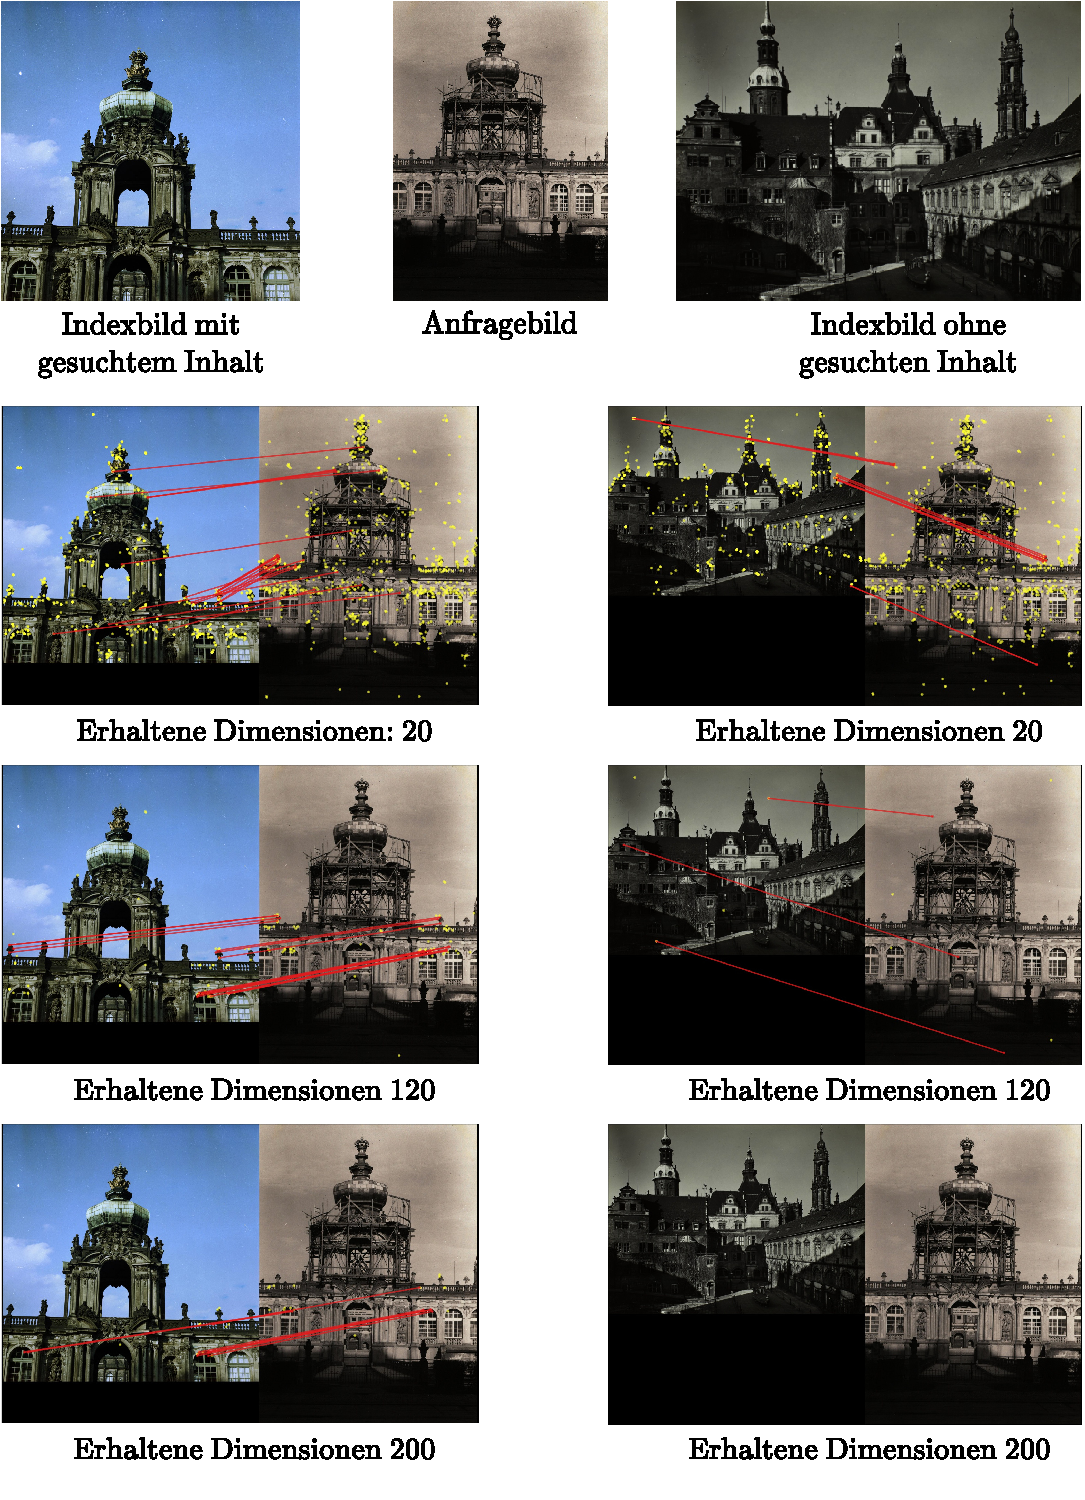
\includegraphics[scale=0.86]{influence_dim}
\caption{Einfluss der Deskriptorlänge auf das Deskriptorenmatching zwischen Anfragebild und Bildern mit und ohne gesuchtem Bildinhalt aus dem Suchindex, bei einem Schwellwert für maximale Deskriptordistanz von $0.8$. Gelbe Punkte markieren Deskriptoren die im Partnerbild gematched wurden. Rote Linien markieren geometrische verifizierte Matches}
\label{influence_dim}
\end{figure}

\begin{figure}[H]
\centering
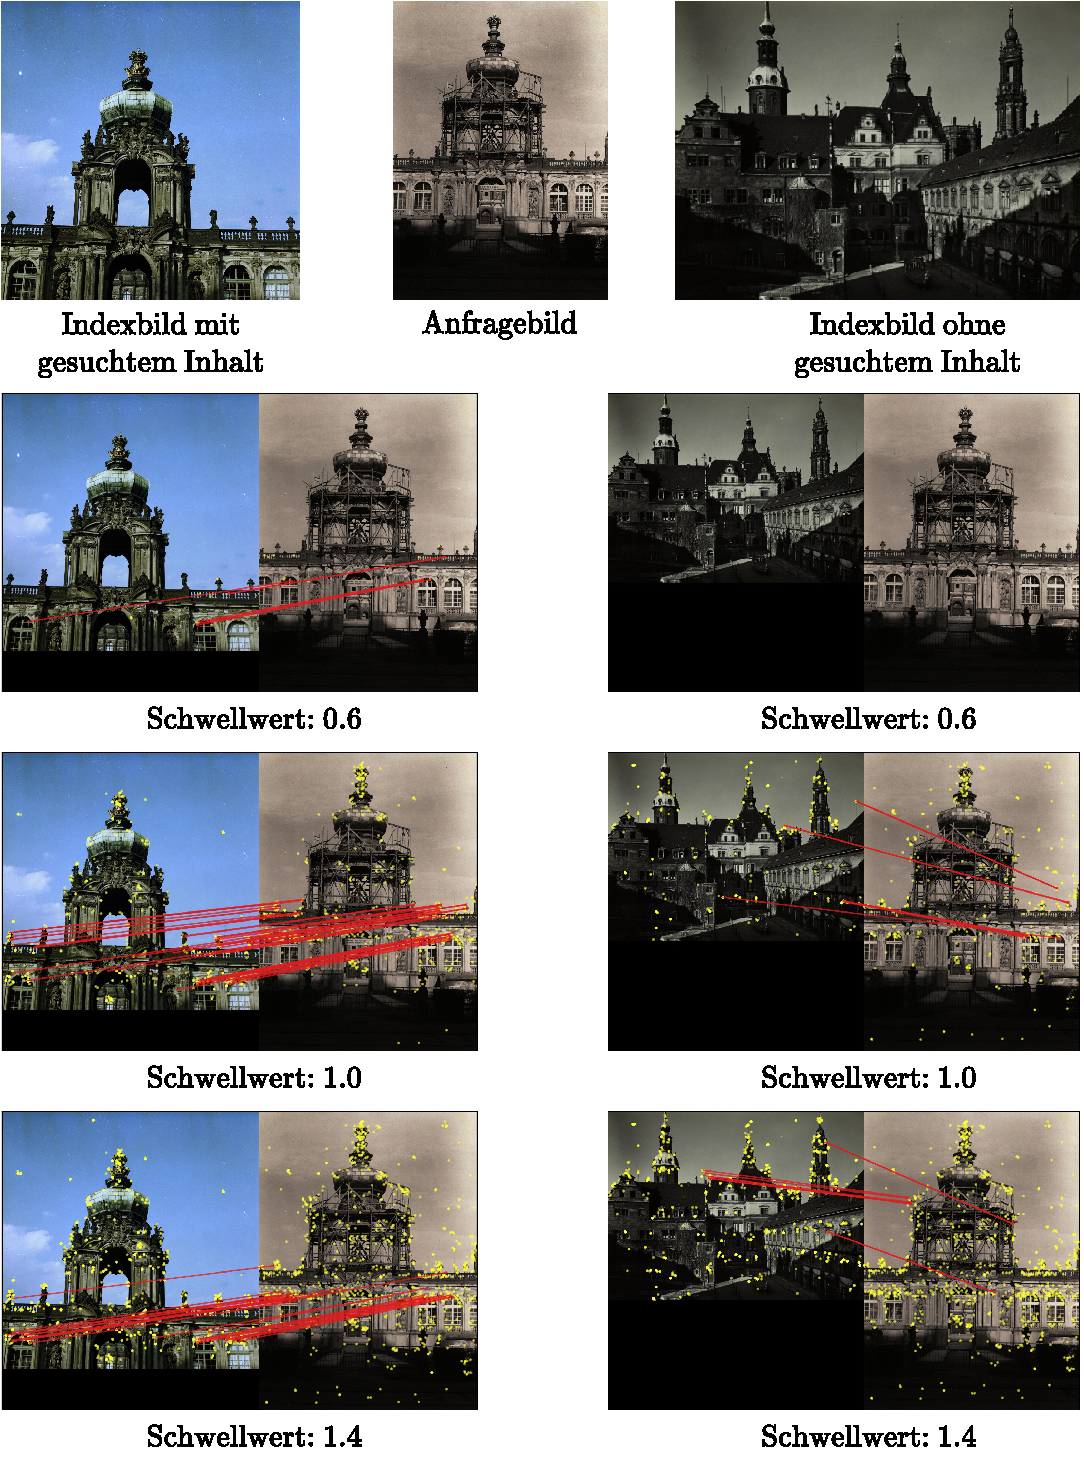
\includegraphics[scale=0.86]{influence_threshold}
\caption{Einfluss des Distanzschwellwerts auf das Deskriptorenmatching, bei Verwendung von $80$ dimensionalen Deskriptoren. Gelbe Punkte markieren Deskriptoren die im Partnerbild gematched wurden. Rote Linien markieren geometrische verifizierte Matches}
\label{influence_threshold}
\end{figure}

Die Autoren der DELF-Papiers \cite{delf} verwenden für $40$-Dimensionale Deskriptoren einen Schwellwert von $0.8$. 
Im Folgenden werden neben diesem Wert sowohl kleiner, wie auch größere Werte zwischen $0.6$ und $1.4$ in Intervallschritten von $0.2$ getestet. Alle Parameterkombinationen von Deskriptorlänge und Distanzschwellwert werden auf den $6$ trainierten Modellen getestet. Für die Auswertung werden die Ergebnisse jeweils über die Läufe der $6$ Modelle gemittelt. Zusätzlich werden Fehlerbereiche im Größer der Standardabweichung angegeben. In Abb. \ref{mAP_num_dim} ist für alle betrachteten Konfigurationen von Deskriptorlänge und Distanzschwellwert, die auf dem historischen Datensatz sowie auf den Oxford5k-Daten getestet werden, die erreichte mAP dargestellt.

\begin{figure}[h]
\includegraphics[scale=0.73]{mAp_num_dim}
\caption{Erreichte mAP bei unterschiedlicher Deskriptorlänge und Distanzschwellwert.}
\label{mAP_num_dim}
\end{figure}

\begin{figure}[h]
\includegraphics[scale=0.73]{mAp_var_dist_ratio}
\caption{Erreichte mAP bei unterschiedlichen Verhältnissen zwischen erklärtem Varianzanteil und gewähltem Distanzschwellwert.}
\label{mAP_var_dist_ratio}
\end{figure}
Unabhängig der getesteten Konfiguration erzielt DELF auf dem Oxford5k-Datensatz eine deutlich höhere mAP als auf den historischen Daten. Welche Aspekte des historischen Datensatzes für das DELF-Verfahren besonders schwierig sind wird anschließend an die Parameterbetrachtung genauer betrachtet. Wie erwartet lassen sich mit größerer Deskriptorlänge bei geeignetem Distanzschwellwert tendenziell bessere Ergebnisse erzielen. Die beste gefundene Konfiguration auf den historischen Daten nutzt Deskriptoren der Länge $160$ bei einem Schwellwert von $1.0$ und erzielt im Mittel eine mAP von $0.57$. Auf Oxford5k erreicht die beste Konfiguration im Mittel eine mAP von $0.71$ und nutzt dabei eine Deskriptorlänge von $120$, mit einen Schwellwert von $1.0$ . Allerdings lässt sich auf Oxford5k mit der von den DELF-Autoren empfohlenen Deskriptorlänge von $40$ und dem empfohlenen Schwellwert von $0.8$ mit einer mittleren mAP von $0.70$ bereits fast gleich gute Ergebnisse erzielen. Lediglich bei Verwendung von noch kleineren Deskriptoren lassen sich signifikante Performanzeinbußen feststellen. So erreicht die beste Konfiguration mit Deskriptorlänge $20$ im Mittel nur eine mAP von $0.65$. Auf den historischen Daten lassen sich mit Deskriptoren mit mehr als $40$ Dimensionen noch signifikante Verbesserungen erzielen. So erreicht die beste Konfiguration mit $80$ Dimensionen eine im Mittel um $0.03$ höhere mAP als die von den Autoren empfohlene Konfiguration. Eine weitere Vergrößerung der Deskriptoren ziehen allerdings auch auf den historischen Daten keine großen Performanzverbesserungen nach sich.
\\
Bei Betrachtung der Distanzschwellwerte, stellt man fest, dass der optimale Schwellwert mit der Länge der verwendeten Deskriptoren steigt. Dies deckt sich mit den Beobachtungen aus Abb. \ref{influence_dim} und Abb. \ref{influence_threshold}, da mit wachsender Deskriptorlänge ein höherer Schwellwert gewählt werden muss, um eine adäquate Anzahl an Deskriptormatches zu erhalten. Bei einem zu klein gewählten Schwellwert werden fast alle potentiellen Deskriptormatches aussortiert, was zu einem drastischen Perfomanzverlust führt. Ein zu groß gewählter Schwellwert führt ebenfalls zu Performanzverlusten, welche jedoch deutlich geringer ausfallen. Das ist der zusätzlichen geometrischen Verifikation mittels RANSAC zu verdanken. Selbst wenn durch den Schwellwert keine unerwünschten Deskriptormatches verworfen werden, wird ein Großteil dieser Matches während der geometrischen Verifikation durch keine Transformation erklärt und so aussortiert\footnote{In Abb. \ref{mAP_num_dim_scoring_methods} auf Seite \pageref{mAP_num_dim_scoring_methods} wird deutlich, dass die Performanz stark unter einem zu hohen Schwellwert leidet, wenn keine geometrische Verifikation durchgeführt wird.}. \\
Wie bereits erläutert hängt die Wahl eines geeigneten Schwellwerts stark von der Länge der Deskriptoren bzw. dem Anteil der von ihnen erklärten Varianz ab. Ein mögliche Strategie für die Untersuchung von vielen unterschiedlichen Deskriptorlänge ist daher den Schwellwert direkt abhängig von der erklärten Varianz zu bestimmen und so die Anzahl zu testender Konfigurationen zu reduzieren. In Abb. \ref{mAP_var_dist_ratio} ist die erreichte mAP im Bezug zum Verhältnis zwischen erklärter Varianz und Schwellwert abgebildet. Tatsächlich erreichen fast alle Deskriptorlängen ihr bestes Ergebnis, wenn das Verhältnis zwischen dem Anteil der erklärten Varianz und dem gewählten Schwellwert zwischen $0.5$ und $0.7$ liegt\footnote{Die wird besonders deutlich, wenn keine geometrische Verifikation stattfindet und zu große Schwellwerte stärkere negative Einflüsse zeigen. Abbildungen hierzu finden sich im Anhang ab Seite \pageref{mAP_var_dist_ratio_alternative_scoring}.}. Für die Untersuchung anderer Deskriptorlängen wäre es daher sinnvoll Schwellwerte zu testen, die innerhalb dieses Bereiches liegen.

\subsection{Alternativen zur Bewertung von Deskriptormatches}\label{metric_experiment}

Bei der Überprüfung auf geometrische Plausibilität von Deskriptormatches mittels RANSAC werden durch Betrachtung der Deskriptorpositionen zusätzliche Informationen für das Matching nutzbar gemacht, die idealerweise Suchergebnisse verbessern. Dabei sollte beachtet werden, dass diese geometrische Überprüfung für einen Großteil der für das Matching benötigten Rechenzeit verantwortlich ist. Im Folgenden wird analysiert, ob und wie stark sich Suchergebnisse unter Verwendung von RANSAC gegenüber alternativen Bewertungsmethoden für Deskriptormatches verbessern, um zu bewerten wie sinnvoll dieser zusätzliche Arbeitsschritt ist.
\\
Eine einfache Möglichkeit um ein Matching ohne geometrische Verifikation zu Bewerten ist die Anzahl an Deskriptormatches zu zählen. Je mehr Deskriptorenpaare zwischen einem Bildpaar gefunden werden können, desto mehr sollte sich der Inhalt dieser Bilder ähneln. Voraussetzung für eine aussagekräftige Bewertung ist die Verwendung eines geeigneten Distanzschwellwertes. Dieser entscheidet, welche Deskriptorpaare keine ausreichende Ähnlichkeit vorweisen können und daher verworfen werden sollten. Paare, die diesen Schwellwert nicht überschreiten gehen alle mit der gleichen Gewichtung in die Bewertung mit ein. 
\\
Intuitiv stellen Deskriptorpaare, die sich besonders stark ähneln, jedoch einen besseren Indikator für die Ähnlichkeit zwischen Bildern dar, als Paare, die diesen Schwellwert nur knapp unterschreiten. Daher wird als weitere Bewertungsmethode eine gewichtete Anzahl an Deskriptorpaaren berechnet. Paare, die den Schwellwert unterschreiten, gehen hierbei mit einem Gewicht zwischen $0$ und $1$ in die Bewertung ein. Ein Paar an identischen Deskriptoren geht dabei mit Gewicht $1$ und ein Paar, dessen Distanz genau dem Schwellwert entspricht, mit Gewicht $0$ in die Bewertung ein. Die Gewichtung verläuft linear antiproportional zur Distanz der Deskriptorpaare. Die gewichtete Anzahl bei Distanzschwellwert $T$ ergibt sich aus,

\begin{equation}
\text{gewichtete Anzahl} = \sum_{i=1}^{|D_\Delta|}{1 - \frac{d_{\Delta i}}{T}},
\end{equation}

Wobei $D_\Delta$ die Distanzen aller Deskriptorpaare $d_{\Delta i}$ enthält, die den Schwellwert nicht überschreiten.
Bei den Experimenten zu Deskriptorlänge und Distanzschwellwert wurden die alternativen Bewertungsmethoden direkt mitberechnet.
\begin{figure}[h]
\includegraphics[scale=0.73]{mAp_num_dim_scoring_methods}
\caption{Erreichte mAP bei unterschiedlicher Deskriptorlänge und Distanzschwellwert unter Verwendung alternativer Bewertungsmethoden.}
\label{mAP_num_dim_scoring_methods}
\end{figure}
In Abb. \ref{mAP_num_dim_scoring_methods} sind die Ergebnisse der alternativen Methoden, analog wie für RANSAC in Abb. \ref{mAP_num_dim} dargestellt.\\
Auch mit alternativen Bewertungsmethoden erzielt DELF auf dem Oxford5k-Datensatz eine deutlich höhere mAP, als auf den historischen Daten. 
Deskriptoren mit mehr Dimensionen erreichen unter Verwendung eines optimierten Distanzschwellwerts eine tendenziell höhere mAP, wobei die Performanzunterschiede auf den historischen Daten deutlich größer ausfallen, als auf dem Oxford5k-Datensatz. Die größte Verbesserung diesbezüglich wird auf den historische Daten erzielt, wenn die Anzahl an Deskriptormatches zur Bewertung verwendet wird (siehe \ref{mAP_num_dim_scoring_methods} a). Hier verbessert sich die durchschnittliche mAP bei einer Erhöhung der Deskriptorlänge von $20$ auf $200$  um $0.09$.\\
Die Verwendung eines sehr kleinen Distanzschwellwertes führt, wie bereits unter RANSAC beobachtet (vgl. Abb. \ref{mAP_num_dim}), zu einer drastischen Verschlechterung der Performanz, unabhängig welche Bewertungsmethode genutzt wird. Bei Wahl eines sehr großen Schwellwertes, der unter Verwendung von RANSAC nur zur geringfügigen Verschlechterungen der Performanz führt, werden deutlich schlechtere Ergebnisse erzielt, wenn die Anzahl der Deskriptormatches zur Bewertung genutzt wird (siehe \ref{mAP_num_dim_scoring_methods} a, b). Je höher der Schwellwert gewählt ist, desto mehr Deskriptorpaare, dessen Deskriptoren keinen ähnlichen Bildinhalt repräsentieren, werden akzeptiert. Da fälschlicherweise akzeptierte Deskriptorpaare gleichermaßen in die Bewertung eines Matchings eingehen, können auch Bildpaare ohne ähnlichem Bildinhalt hoch bewertet werden. Ab einem gewissen Punkt kann in jedem Bildpaar für jeden Deskriptor ein Partner gefunden werden. Somit erhält jedes Bildpaar die gleiche Bewertung, wodurch Anfragen mit Bildern in einer zufälligen Reihenfolge beantwortet werden. Werden die Deskriptorpaare nach ihrer Ähnlichkeit gewichtet (siehe \ref{mAP_num_dim_scoring_methods} c, d), gehen Deskriptorpaare, die sehr unterschiedliche Bildinhalte repräsentierten, deutlich schwächer in die Bewertung ein, weshalb sich ein zu großer Schwellwert kaum negativ auf Ergebnisse auswirkt.
\\
\begin{figure}[h]
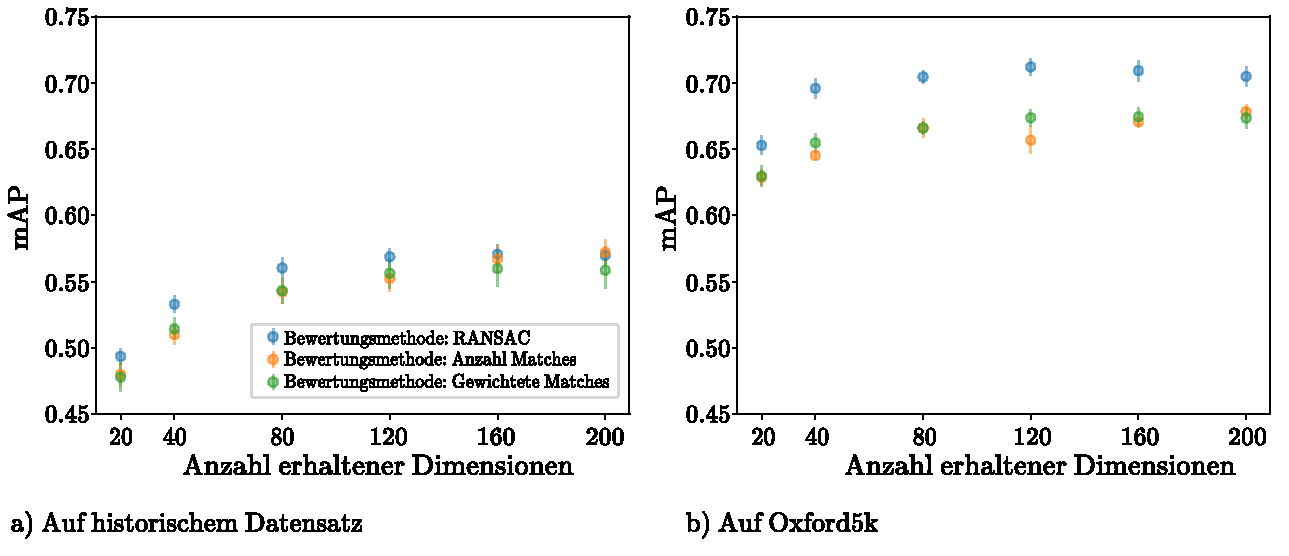
\includegraphics[scale=0.74]{compare_scoring_methods}
\caption{Erreichte mAP bei unterschiedlicher Deskriptorlänge mit optimiertem Distanzschwellwert unter Verwendung unterschiedlicher Bewertungsmethoden.}
\label{compare_scoring_methods}
\end{figure}
Wie sich die Performanz, je nach gewählter Bewertungsmethode und Deskriptorlänge unterscheidet ist in Abb. \ref{compare_scoring_methods} dargestellt. Die hier gezeigten Konfigurationen verwenden jeweils die besten für sie gefundenen Schwellwerte. Auf den Oxford5k-Daten werden mit RANSAC deutlich bessere Ergebnisse, als mit anderen Bewertungsmethoden erzielt. Die beste gefundene Konfiguration erreicht dabei im Mittel eine mAP von $0.71$. Die beste Konfiguration mit einer alternativen Bewertungsmethode nutzt die Anzahl Matches zur Bewertung und erreicht eine mittlere mAP von $0.68$. Die Ergebnisse bei Betrachtung von gewichteten Matches unterscheidet sich dabei kaum von den Ergebnissen basierend auf der reinen Matchanzahl.
\\
Auf den historischen Daten fallen die Verbesserungen durch RANSAC deutlich geringer aus. Insbesondere bei Verwendung von hochdimensionalen Deskriptoren werden durch geometrische Verifikation keine besseren Ergebnisse erzielt, als bei Verwendung der Matchanzahl. Die beste gefundene Konfiguration für die historischen Daten nutzt ebenfalls die Anzahl an Matches zur Bewertung und erzielt eine mittlere mAP von $0.57$. Die Unterschiede zur besten RANSAC-Konfiguration liegen jedoch innerhalb der ermittelten Fehlerbereiche. Die Betrachtung anhand gewichteter Matches schneidet auch auf den historischen Daten größtenteils ähnlich wie die Betrachtung anhand der Anzahl an Matches ab. Lediglich bei sehr Verwendung sehr großer Deskriptoren werden im Vergleich schlechtere Ergebnisse erzielt. Speziell für den historischen Anwendungsfall scheint der zusätzliche geometrische Verifikationsschritt keinen signifikanten Verbesserungen der Performanz zu erzielen.
Um genauer einzugrenzen, auf welchen Daten RANSAC in der Lage ist Retrievalergebnisse zu verbessern, und wo dies nicht funktioniert, ist in Tab. \ref{scoring_mAP_change_by_category} für die unterschiedlichen Anfragekategorien aufgeführt, wie sich die mAP bei Verwendung von RANSAC gegenüber der Bewertung mittels Matchanzahl verändert.
\\
\begin{table}[]
\setlength\tabcolsep{0pt}
\resizebox{\textwidth}{!}{%
\begin{tabular}{cccccccc} 

\large{Kategorie}                          & \large{Frauenkirche}                    & \large{Hofkirche}                       & \large{Zwinger}                         & \large{Sophienkirche} & \large{Semperoper} & \large{Moritzburg} & \large{Stallhof} \\
&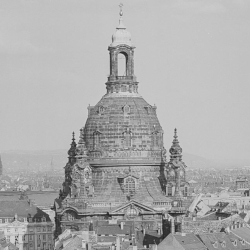
\includegraphics[scale=1.4]{category_thumbs/frauenkirche_thumb}&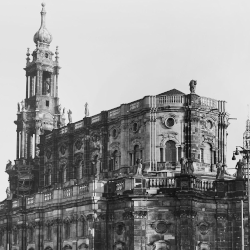
\includegraphics[scale=1.4]{category_thumbs/hofkirche_thumb} &      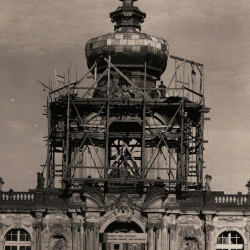
\includegraphics[scale=1.4]{category_thumbs/zwinger_thumb}&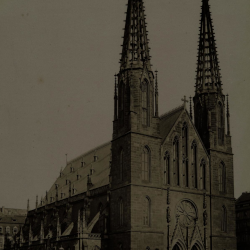
\includegraphics[scale=1.4]{category_thumbs/sophienkirche_thumb}&     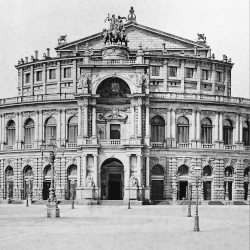
\includegraphics[scale=1.4]{category_thumbs/semperoper_thumb}&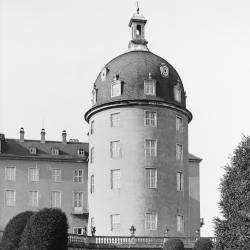
\includegraphics[scale=1.4]{category_thumbs/moritzburg_thumb}&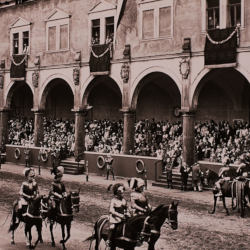
\includegraphics[scale=1.4]{category_thumbs/stallhof_thumb}                    \\
\large{$\Delta$mAP} & \large{$0.076$} & \large{$0.076$} & \large{$0.025$} & \large{$-0.011$} & \large{$-0.034$} & \large{$-0.074$} & \large{$-0.153$}\\              
\end{tabular}
}
\setlength\tabcolsep{6pt}
\caption{Veränderung der mAP bei Verwendung von RANSAC gegenüber einfachem zählen der Deskriptormatches, je nach Objektkategorie. Der betrachtete Testlauf verwendet eine Deskriptorlänge von $200$ und einen Distanzschwellwert von $1.0$.}
\label{scoring_mAP_change_by_category}
\end{table}
Dabei zeigt sich, dass Motive mit gut differenzierbaren markanten Bereichen, wie beispielsweise die Türme der Frauenkirche stark von einer geometrischen Verifizierung profitieren. Objekte die häufig wiederkehrende Elemente enthalten, wie zum Beispiel die Fenster der Moritzburg oder die Arkaden des Stallhofs, verschlechtern sich dagegen bei Verwendung von RANSAC.
\\
\begin{figure}[h]
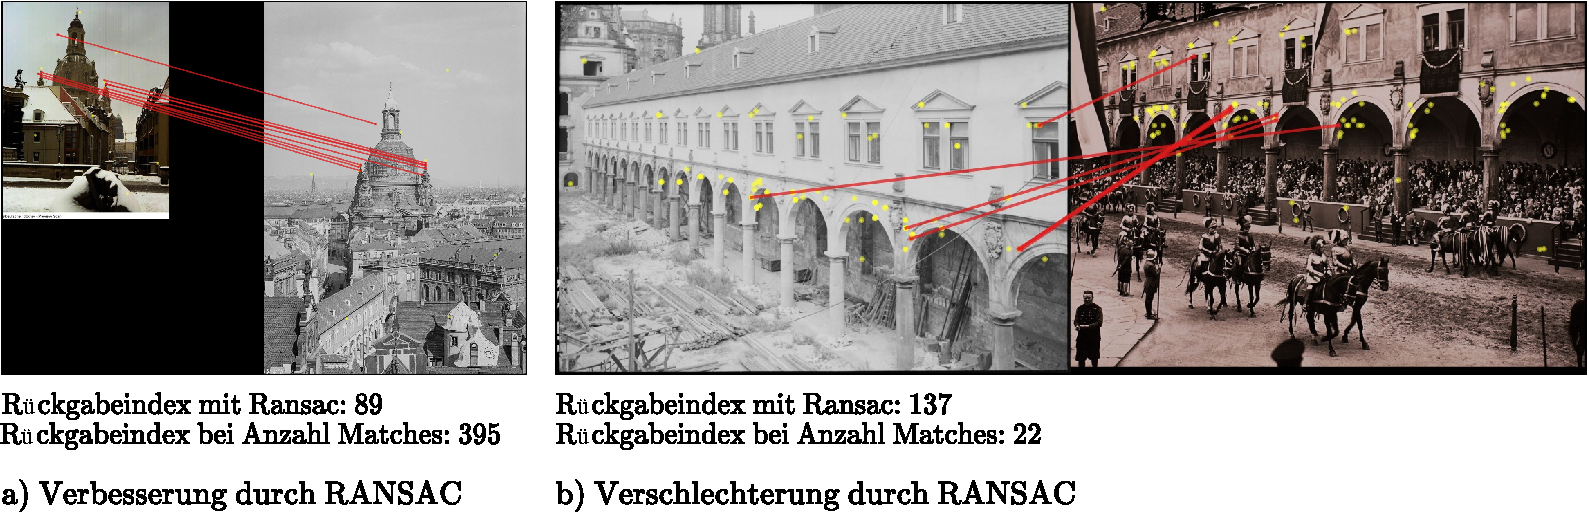
\includegraphics[scale=0.595]{where_ransac_shines}
\caption{Beispiele für Matchings von Bildpaaren mit gleichem Bildinhalt, die von geometrischer Überprüfung profitieren, bzw. darunter leiden. Der Rückgabeindex gibt an, an wievielter Stelle der Anfrageantwort das entsprechende Bildpaar zurückgegeben wird (niedriger ist besser). Gelbe Punkte repräsentieren Deskriptoren, für die ein Match gefunden wurde. Rote Linen verbinden verifizierte Deskriptorpaare.}
\label{where_ransac_shines}
\end{figure}

Warum die geometrische Überprüfung hier problematisch ist lässt sich gut an dem Beispielmatching zweier Stallhofbilder in Abb. \ref{where_ransac_shines} b erkennen. Obwohl DELF viele Matchpaare entlang der Arkaden und Fenstern findet, können nur wenige mit einer affinen Transformation erklärt werden. Betrachtet man die verifizierten Matches, so fällt auf, dass DELF Schwierigkeiten hat die korrekten Arkaden miteinander zu matchen. Auf Grund der sich wiederholenden Strukturen, können einzelne Bereiche nicht klar genug unterschieden werden. Das resultierende Matching lässt sich daher nicht einheitlich mit einer Transformation erklären. Im Gegensatz dazu konzentriert sich das Beispielmatching der Frauenkirche (vgl. Abb. \ref{where_ransac_shines} a) nur auf zwei ihrer seitlichen Türme, wodurch sich eine Transformation finden lässt, die einen Großteil der Deskriptorpaare erklärt. Obwohl hier die Anzahl der Deskriptorpaare vergleichsweise gering ist, kann durch die geometrische Verifikation ein gutes Matching erstellt werden.
\\
Abschließend lässt sich zusammenfassen, dass der zusätzliche Verifikationsschritt, den DELF vorschreibt, nicht uneingeschränkt sinnvoll für das lösen von Retrievalaufgaben ist. Architektonische Besonderheiten und Beschaffenheit der Bildinhalte haben einen signifikanten Einfluss auf Effektivität von RANSAC, somit sollte der Einsatz, je nach Datensatz überdacht werden. Um herauszufinden, ob RANSAC allgemein für die historische Domäne ungeeignet ist, sollten jedoch weiter Experimente auf einem erweiterten Datensatz, insbesondere mit mehr unterschiedlichen Motiven, durchgeführt werden.


\subsection{Alternative Extraktionspunkte}

Das DELF-Verfahren sieht es vor, die Ausgaben des dritten Blocks aus dem zugrundeliegenden ResNet-50 (vgl. Abb. \ref{resnet}b auf Seite \pageref{resnet}) als Deskriptoren zu verwenden. Warum genau dieser Punkt zur Extraktion der Deskriptoren verwendet wird, begründen die Autoren des DELF-Papiers \cite{delf} jedoch nicht. Als letzte Parameterbetrachtung dieser Arbeit wird daher ein alternativer Extraktionspunkt untersucht. Dabei werden die Netzwerkausgaben des vierten und letzten ResNet-Blocks betrachtet. Diese Wahl beruht auf den Beobachtungen von Zeiler und Fergus, die in \cite{extraction_point_meaning} gezeigt haben, dass Netzwerkausgaben aus späteren Schichten eines neuronalen Netzes in der Lage sind komplexere Bildmerkmale detektieren. Deskriptoren aus dieser späten Schicht können daher möglicherweise besser für die Differenzierung komplexer Bildinhalte genutzt werden.
\\
Die bisher verwendeten Extraktionsnetzwerke können für die Deskriptorextraktion aus Block-4 weiter verwendet werden. Da sich die extrahierten Deskriptoren jedoch in Form und Inhalt von Deskriptoren aus Block-3 unterscheiden, müssen für die Deskriptorauswahl neue Attention-Netzwerke trainiert werden. Zunächst findet hierfür eine Optimierung der Hyperparameter analog wie in Kap. \ref{hyperparam} statt. Es zeigt sich dabei, dass alle Testläufe unabhängig ihrer Hyperparameterkonfigurationen, ähnlich gute Testergebnisse erzielen\footnote{Grafiken zu dieser Hyperparameteroptimierung finden sich im Anhang ab Seite \pageref{hyperopt_layer4}.}. Mit den optimierten Hyperparametern werden anschließend $6$ neue Attention-Modelle trainiert. Die Trainingsverläufe dieser Modelle (siehe Abb. \ref{optimized_runs_layer4}) erreichen bereits ab der ersten Epoche sehr hohe Validierungsgenauigkeiten und steigern sich während des Trainings auch nur geringfügig. Im Vergleich dazu zeigen Trainingsverläufe auf Basis von Deskriptoren aus Block-3 eine sehr geringe initiale Validierungsgenauigkeit, die sich während des Trainings deutlich steigert (siehe Abb. \ref{optimized_runs} b auf Seite \pageref{optimized_runs}). 
\begin{figure}[h]
\centering
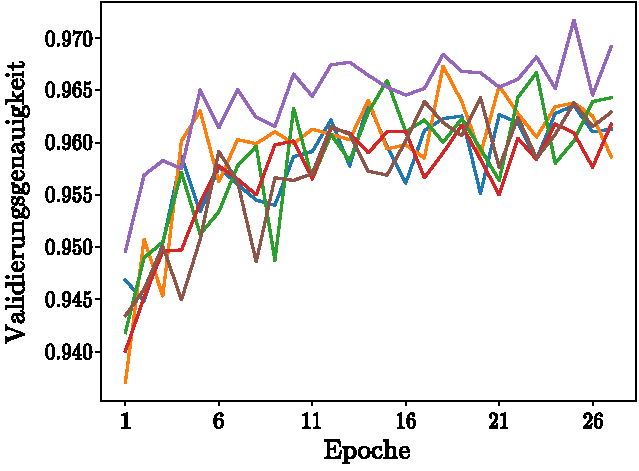
\includegraphics[scale=1]{NNOPT/6_model_verlauf_layer4}
\caption{Verläufe des Attention-Trainings für Deskriptoren aus Block-4, mit optimierten Hyperparametern.}
\label{optimized_runs_layer4}
\end{figure}
Die Ausgaben aus dem vierten Block gehen während des Fine-Tunings, nach einem finalen Pooling direkt in die Klassifikationsschicht ein. Es ist also nicht verwunderlich, dass diese Ausgaben auch vom Attention-Netzwerk sehr effizient genutzt werden können, um Klassifikationsaufgaben zu lösen. Fraglich ist dabei, ob die vom Attention-Netzwerk gelernte Gewichtung bzw. Auswahl der Deskriptoren für eine erfolgreiche Klassifikation entscheidend ist, oder ob auf Grund der aussagekräftigen Deskriptoren eine beliebige Auswahl an Deskriptoren genügt, um die Klassifikationsaufgabe zu lösen. Falls die Gewichtung der Deskriptoren für da Training nur geringe Auswirkungen zeigt, könnte sich dies negativ auf die gelernte Selektionsfähigkeit des Attention-Netzwerks auswirken.
\\


\begin{figure}[h]
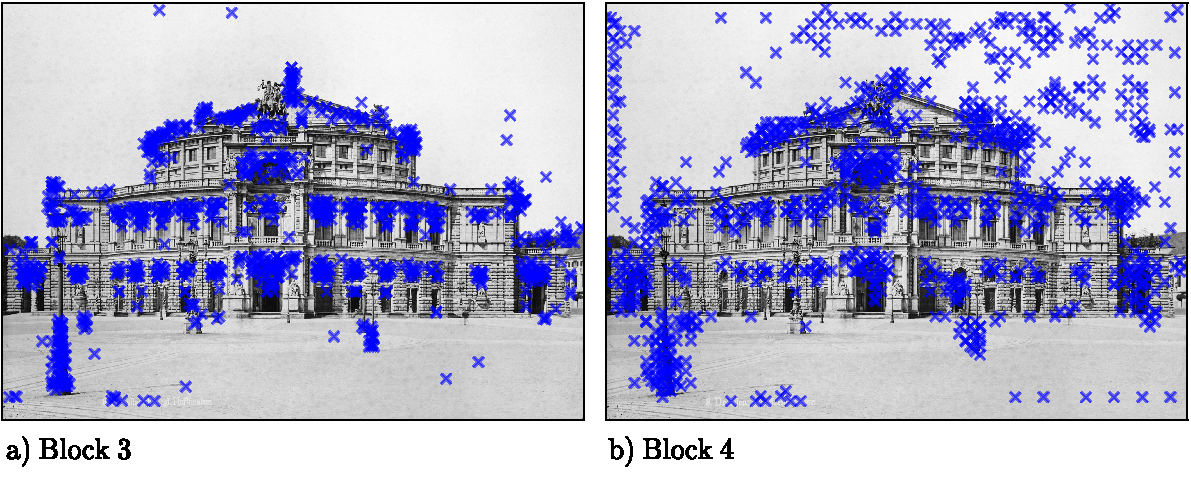
\includegraphics[scale=0.73]{attention_layer_diff}
\caption{Unterschiede der Deskriptorselektion bei Verwendung unterschiedlicher Extraktionspunkte.}
\label{attention_layer_diff}
\end{figure}
In Abb. \ref{attention_layer_diff} ist das Auswahlverhalten der Attention-Netzwerke bei unterschiedlichen Extraktionspunkten, an dem Beispiel eines Bildes der Semperoper, dargestellt. Es zeigt sich, dass das Attention-Netzwerk auf Basis der Deskriptoren aus Block-4 deutlich mehr Deskriptoren außerhalb der Semperoper selektiert.
Ein Aspekt, der die Auswahl von Deskriptoren außerhalb der interessanten Bildbereiche begünstigt ist, dass bei der Verwendung eines späteren Extraktionspunktes, auf Grund der Netzwerkarchitektur, eine geringere Anzahl an Deskriptoren erzeugt wird. Die negativen Auswirkungen einer geringen Auswahl an Deskriptoren wurde bereits in Abb. \ref{small_img} auf Seite \pageref{small_img} beobachtet\footnote{Bei einer Extraktion nach Block-4 werden ca. $75 \%$ weniger Deskriptoren erzeugt, als bei Block-3. Im Vergleich dazu werden nach einer Skalierung von der Originalgröße($2.5$ MPixel) auf $0.6$ MPixel, wie in Abb. \ref{small_img} dargestellt, ca. $76 \%$ weniger Deskriptoren erzeugt. Die Deskriptorauswahl auf der $0.6$ MPixel Version scheint jedoch deutlich besser zu funktionieren, als mit Deskriptoren aus Block-4 in Originalgröße. Folglich scheint die Anzahl an erzeugten Deskriptoren nicht alleiniger Grund für das schlechter Auswahlverhalten zu sein.}. 

 
